\newchapter{commissioning}{Setup and Commissioning of the PFF System}

The function of the phase monitor electronics has already been introduced in Chapter~\ref{c:phaseMons}. This chapter discusses the design, setup and performance of the remaining PFF hardware --- the FONT5a board and the kicker amplifiers. The second part of the chapter then presents remaining measurements that had to be taken to commission the PFF system, such as setting up the correction timing and verifying the ability to shift the phase in the TL2 chicane using the kickers and PFF optics.

Figure~\ref{f:racks} shows the complete PFF electronics setup in the klystron gallery, consisting of three racks. The cables from the phase monitors and kickers in the accelerator hall on the floor below enter the rack from behind. They are connected to the patch panels at the lower left side of the figure, for the phase monitors, and below the amplifier in the middle rack, for the kickers. Signals are then directed from the patch panels to the relevant pieces of hardware in the PFF chain. 

\begin{figure}
  \centering
  \includegraphics[width=\textwidth]{Figures/commissioning/racks}
  \caption{The PFF system electronics racks. Each major component of the system is labelled, including the phase monitor electronics, FONT5a board and kicker amplifier.}
  \label{f:racks}
\end{figure}

\newsection{fontSetup}{Feedforward Controller (FONT5a Board)}

This section describes the design, fimrware and operational aspects of the FONT5a board, which acts as the PFF controller. Its role is to digitise the signals from the first upstream phase monitor (Mon~1), process them and calculate the appropriate voltage with which to drive the kicker amplifiers in order to correct the phase downstream. In addition it must ensure the timing of the correction output is such that the drive output from the amplifiers reaches the kickers precisely in time with the beam.

The FONT5a board is a custom built digital board designed and constructed by the FONT group at Oxford University \cite{fontGroup}. More details of the design of the board and the internal components can be found in \cite{dougThesis}. It was initially built as the controller for prototypes of an IP (interaction/beam collision point) position feedback for future linear colliders, either ILC or CLIC. Tests of this feedback are ongoing at ATF2, KEK in Japan  \cite{ipfbIPAC16}. At the heart of the FONT5a board is a Xilinx Virtex-5 field programmable gate array (FPGA) \cite{xilinx}, an integrated circuit with customisable logic that the user can program as desired for his or her application. Exactly the same hardware can therefore be used for the PFF and IP feedback controllers, with different firmware loaded on to the FPGA to take in to account the different signal processing required for the input and output signals in each application.

An annotated picture of the FONT5a board front panel is shown in Figure~\ref{f:FONT5aPanelPic}. Apart from the FPGA (inside the board and therefore not seen in the figure) the main components of the FONT5a board are nine analogue to digital converters (ADCs) and four digital to analogue converters (DACs). In addition there is a serial RS232 port used to communicate with a LabVIEW data acquisition and control system (DAQ), a JTAG connector used to program the firmware on the FPGA should it need to be changed, and several other inputs and outputs mostly used for the timing and triggering of the board.

The outputs from the phase monitor electronics, mixer and diode signals, are connected to the ADC inputs on the FONT5a board. Usually only the Mon~1 outputs are connected to the FONT5a board, with the diode on ADC~1 and the mixer on ADC~2, although the signals from additional monitors can be connected if needed. The ADCs are 14-bit with an input range of \(\pm0.5\)~V. Due to the expected noise on the ADCs the least significant bit is discared and only the most significant 13 bits are processed by the FPGA \cite{fontPaper}. The processed ADC outputs therefore have a range of \(\pm4096\) values or ``counts'', corresponding to 0.12~mV per ADC count. More details on the digitisation of the phase monitor signals were given in Section~\ref{s:monDigitisers}. 

Each ADC output can have a non-zero mean voltage in its baseline noise. To be able to remove these intrinsic voltage offsets each analogue input is combined with the output from a DAC, labelled ``trim DACs'' (separate from the DACs used as the PFF correction outputs). By varying the trim DAC voltages it can be ensured that the baseline output of each ADC is 0~V, so that its full \(\pm0.5\)~V range can be used for the signal of interest.

For the PFF system the ADCs are usually clocked at a sampling rate of 357~MHz, generated by an external clock generator \cite{srsClockGen} and connected to the ``FST CLK'' input on the FONT5a board. 357~MHz is used for historical reasons, as this is the sampling rate for which experience has been gained for the IP feedback applications. The start of the ADC sampling window is determined by an external 0.8~Hz trigger derived from the CTF3 timing and therefore locked to the beam. The trigger is connected to the ``DIG IN B'' input on the board, and arrives 17~\(\mathrm{\mu s}\) before the beam to take in to account the ADC warmup time.

After being processed on the FPGA the calculated correction outputs are sent to the DAC outputs, which are 14-bit with an output range of \(\pm2\)~V to match the required range for the input of the PFF kicker amplifiers. Only DAC~1 and DAC~2 are used for the PFF system, the other two DACs are unused. In addition the FONT5a board generates the trigger for the amplifier, which is sent from the ``AUX OUT A'' output and must arrive at the amplifier 1.5~\(\mathrm{\mu s}\) before the DAC output signals.

\begin{figure}
  \centering
  \includegraphics[width=0.9\textwidth]{Figures/commissioning/FONT5aPanelPic}
  \caption{Front panel of the FONT5a board. All the connectors relevant to PFF operation are highlighted, the remaining connectors are not used at CTF3. All connectors are BNC apart from the power connector, RS232 serial port used to communicate with the LabVIEW data acquisition system (DAQ) and the JTAG connection used to program the firmware on the FPGA. The use of the ADCs, DACs and timing (trigger and clock) connections is summarised in Figure~\ref{f:fontDiagram}. }
  \label{f:FONT5aPanelPic}
\end{figure}

Finally, the FONT5a board is controlled using a LabVIEW data acquisition system (DAQ) documented in \cite{dougThesis}, with communication between the board and the DAQ via the serial RS232 port. An example screenshot from the DAQ is shown in Figure~\ref{f:DAQScreenshot}. It provides functionality to change all the setup parameters in the FONT5a firmware for the PFF system setup, view the current ADC inputs and DAC outputs in real time and to save data directly from the FONT5a board. However, as the FONT5a board and DAQ currently run as a standalone system at CTF3, PFF data is usually saved via the CERN control system and SiS digitisers where data from other devices, such as BPMs, can be saved in sync with the phase monitor signals as discussed in Section~\ref{s:monDigitisers}. The DAQ runs on a Windows PC next to the racks used for the phase monitor electronics, FONT5a board and amplifier. The PC can be connected to via remote desktop to allow the FONT5a board to be controlled in the CTF3 control room.

\begin{figure}
  \centering
  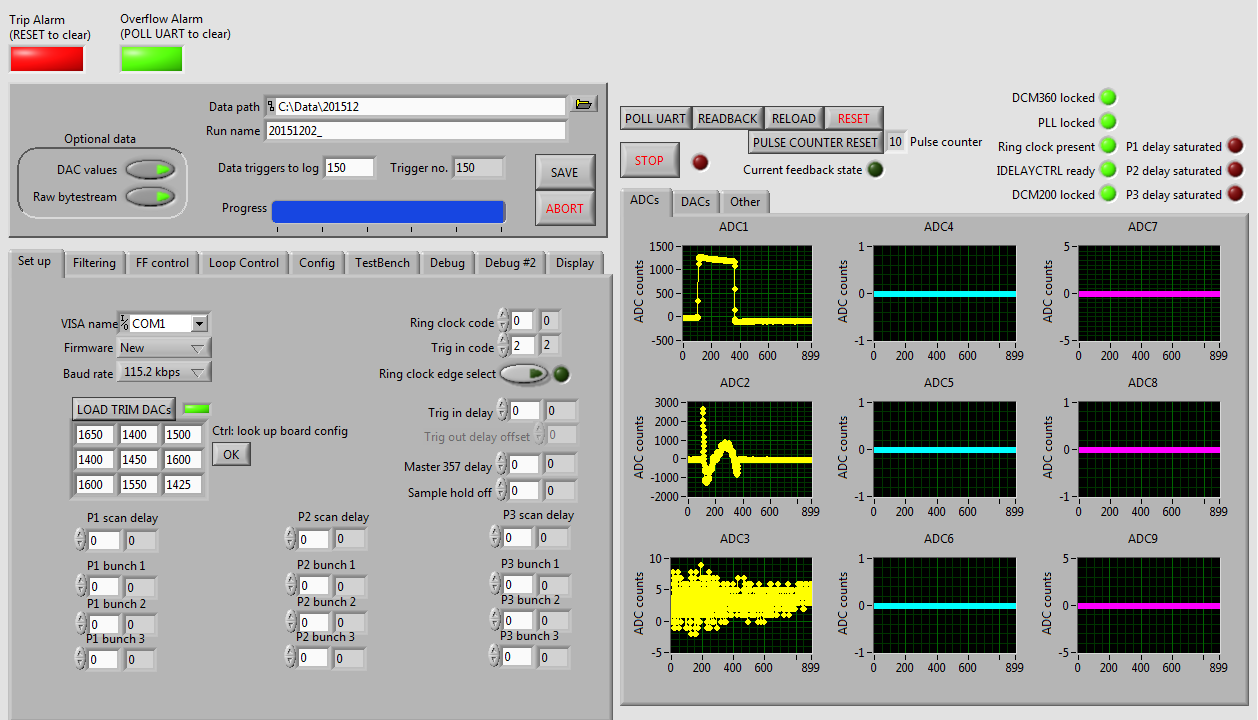
\includegraphics[width=0.8\textwidth]{Figures/commissioning/DAQScreenshot}
  \caption{Screenshot of the LabVIEW DAQ used to control the FONT5a board when setting up the PFF system. The right panel shows plots of the current ADC and DAC outputs. Parameters for the correction can be changed in the left panel.}
  \label{f:DAQScreenshot}
\end{figure}

\subsection{Implementation of PFF Correction}
\label{ss:pffFirmware}

The diagram in Figure~\ref{f:fontDiagram} shows all the connections to and from the FONT5a board that were introduced in the previous section, from the phase monitor and timing inputs on the left side of the diagram to the outputs for the amplifier and DAQ on the right side of the figure. The central portion of the figure shows a simplified version of how the FONT5a firmware calculates and applies the PFF correction. All the parameters shown in the figure, and several others not shown in the diagram but described later in this section, must be correctly set (via the DAQ) for operation of the PFF system.

The basic logic of the firmware is as follows. The ADC timing, sampling rate and start time, are determined by the input trigger and external 357~MHz clock. Duiring the set sampling window the ADC outputs are processed, including a number of channel offsets and filters. The processed ADC~2 (Mixer) output is then split in to two, to create the two strands that become the DAC~1 and DAC~2 outputs. Note that as the Mixer is used directly (rather than \(\arcsin(\mathrm{Mixer})\)) this uses the small angle approximation. The effect of this is discussed in Section~\ref{ss:fontSmallAng}. If the diode (ADC~1) is being used in the calculation the ADC~2 output is also multiplied by 1/sqrt(ADC~1), with values taken from a lookup table rather than being calculated directly to save latency \cite{glennCLIC13}. Prior to being sent to the DACs the two output strands are multiplied by set gain factors and then can be delayed by a set amount of time. The two calculated DAC outputs are then connected to the signal inputs on the amplifiers, where they are amplified and eventually sent to the kickers to deflect the beam and correct the phase. Meanwhile the input trigger for the FONT5a board is used to derive the trigger for the amplifier, with a variable delay that can also be set in the DAQ. The overall latency of the FONT5a board, from the arrival of the signal at the ADCs to the output of the calculated correction at the DACs, is around 22 clock cycles (at 357~MHz) or 60~ns \cite{glennCLIC14}.

\afterpage{\begin{landscape}
\begin{figure}
  \centering
  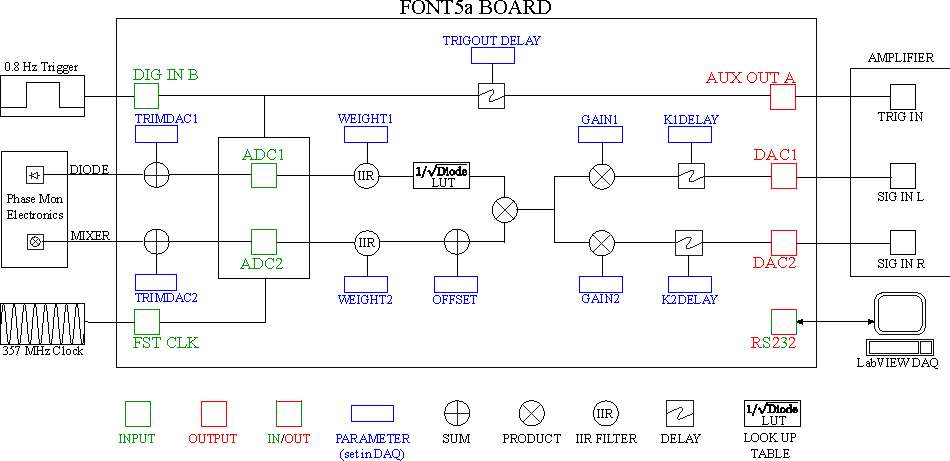
\includegraphics[width=\hsize]{Figures/commissioning/fontDiagram}
  \caption{Schematic of connections to and outputs from the FONT5a board, as well as the PFF calculation in firmware in the case where the diode is used. If the diode is not used the ADC1 input is not required. }
  \label{f:fontDiagram}
\end{figure}
\end{landscape}}

All the parameters and controls that must be adjusted during the PFF system setup, and their respective values where relevant, are listed below for reference. These are only introduced in brief here, but parameters that are either non-trivial to derive or are critical for the PFF performance are described in more detail in later sections and chapters as indicated. The values given are in the units as they are set in the DAQ and firmware, with each parameter expressed by up to a 14~bit number, and the size of each control chosen to give a reasonable degree of flexibility around the expected set point. 

\subsubsection{Input Timing}

The following parameters must be adjusted in order to set the properties of the ADC sampling as desired:

\textbf{Trig in delay:} The Trig in delay allows the start of the ADC sampling window to be delayed with respect to the arrival of the external trigger. The timing of the trigger and correction outputs to the amplifier (Trig out delay and K1/K2 delay) are relative to this delay, therefore changing the Trig in delay value does not effect the synchronisation of the correction output with the beam. The only requirement is to ensure that the full acquired upstream phase monitor signals arrive within the sampling window, and that the trigger arrives early enough to account for the 10~\(\mathrm{\mu}\)s warmup time of the ADCs \cite{glennPriv}. The trigger is set to arrive 17~\(\mathrm{\mu}\)s before the beam, so a trig in delay of around 2500 clock cycles of 357~MHz, or 7~\(\mathrm{\mu}\)s, is used to define the time at whcih the ADCs are turned on (with them then ready 10~\(\mathrm{\mu}\)s later when the beam arrives).

\textbf{Enabled channels:} The FONT5a board has 9~ADCs but only two are usually needed for the PFF system (for the mixer and diode of Mon~1 connected to ADC1 and ADC2, with the other two monitors normally connected to the SiS digitisers, see Section~\ref{monDigitisers}). To avoid hitting the limits of the baud rate  of the RS232 port on the PC the remaining ADC channels can be disabled so their data is not transmitted.

\textbf{No. samples:} The length of the ADC sampling window, in number of samples, can also be varied. Typically 900~samples are used, covering a time window of \(2.5~\mathrm{\mu}\)s with the 357~MHz clock. If the signal from more than two ADCs is needed the number of samples can be reduced to avoid hitting the baud rate limit of the RS232 port on the PC, the only requirement is that the time window is long enough to encompass the full \(1.1~\mathrm{\mu}\)s beam pulse length.

\subsubsection{ADC Signal Processing}

The following parameters must be correctly set in order to remove offsets and droop in the ADC outputs:

\textbf{Trim DACs:} As mentioned in Section~\ref{s:fontSetup} the FONT5a board includes trim DACs in order to remove intrinsic voltage offsets in the output of each ADC. The trim DAC output is added to the ADC inputs, and each trim DAC value must be set correctly in the DAQ. For ADC1 (Diode) and ADC2 (Mixer) the Trim DAC values are 1650 and 1400 counts, corresponding to 8~mV and 7~mV \cite{dougThesis}, respectively.

\textbf{Filter Weights:} Infinite Impulse Response (IIR) filters are implemented in the FONT5a firmware in order to remove droop in the ADC response, see Section~\ref{ss:droopCorr}. The filter weights for each ADC can be adjusted in the DAQ. The correct values are 50 for ADC1 (Diode) and 56 for ADC2 (Mixer).

\textbf{Channel Offset:} To maximise the effect of the PFF system it is necessary to zero the mean upstream mixer (ADC2) output in the central region of the pulse where the correction is being attempted (the start and end of the pulse can not be fully corrected due to the large phase sag, so the central portion is usually used). Ideally this should be adjusted by varying the Mon1 phase shifter, but this can not be done remotely so the channel offset on the FONT5a board can be used instead to make small adjustments from the control room. The channel offset adds a static offset in counts to the ADC2 output, allowing the mixer output to be zeroed at any point along the pulse. The consequences of using a non-optimal Channel Offset are discussed in Section~\ref{ss:longFF_upDrifts}. For large phase offsets giving close to maximum mixer output the phase monitor resolution is degraded (Section~\ref{ss:resVsShifter}) and the small angle approximation used in the FONT5a phase reconstruction (Section~\ref{ss:fontSmallAng}) becomes invalid, in which case the phase shifter should still be used to zero the phase. 

\subsubsection{Output Mode}

The following parameters control the nature of the DAC output signals:

\textbf{Feedforward enable:} The DAC output can be enabled or disabled, as required.

\textbf{Interleaved mode:} With interleaved mode enabled the DAC outputs from the FONT5a board are only sent for half of the triggers, for example being applied to all the odd pulses but not sent for all the even pulses. This is incredibly useful for interpreting the PFF results, as well as being used for many of the other tests presented in this thesis, as it allows a comparison between beam conditions with and without an applied kick at the same time. In this case the effects of any slow drifts should be equivalent in both the kicked and non-kicked data, thus any differences between the two should be a real effect of the PFF system. Data with the DAC output disabled can also be used to simulate the expected effect of the PFF system in those conditions. All the PFF results in Chapter~\ref{c:feedforward} use interleaved data.

\textbf{DAC Output Mode:} The DAC output to the amplifier can be sent in two modes --- Sample-by-sample or Constant DAC. In Sample-by-sample mode the DAC output is as needed for the PFF system, being shaped along the pulse by the measured phase multiplied by the set gain as shown in Figure~\ref{f:fontDiagram}. In Constant DAC output mode a constant output voltage can be sent to the amplifier across the full length of the ADC sampling window (or for a shorter time with an applied gate, see below). The majority of the results presented in the remainder of this chapter use constant DAC outputs for verification of the amplifier, optics, correction range and correction timing.

\textbf{K1, K2 const DAC}: In constant DAC mode the DAC output can be varied between \(\pm4096\)~counts, or \(\pm2\)~V sent to the amplifier, and can be changed independently for each output.

\textbf{Gain}: In sample-by-sample mode the PFF gain can also be set independently for each correction output, with each being a 14-bit value (\(\pm8192\)~units). The conversion between the gain in the units set in the DAQ and the actual applied gain is derived in Section~\ref{ss:pffFirmware}. An applied gain of 624~units corresponds to a real gain of approximately 1 (with a gain of 624 an upstream phase offset of 1~degree corresponds to a downstream phase correction of approximately -1~degrees).

\textbf{Diode Mode:} The FONT5a firmware provides three modes for the treatment of the diode signal on ADC1 --- normalisation, gating and unused. With diode normalisation enabled the PFF system reconstructs the phase as originally envisaged using Mixer/sqrt(Diode). Due to the issues with the phase monitor diodes as discussed in Chapter~\ref{c:phaseMons} the option to not include the diode in the PFF calculation and only include the mixer was later added, which is now the nominal setup. Rather than leaving the diode completely unused, it is usually used to gate the correction output (see below).

\textbf{Overflow Mode:} The PFF correction output can behave in three ways in the case where the calculated output is outside the maximum range of \(\pm4096\)~DAC counts. In the first iteration of the PFF firmware the calculated correction output would overflow, causing sign flips in the output in the regions where the correction range was exceeded \cite{glennPriv}. This behaviour can still be applied in the current firmware if desired. However, in normal operation the output is set to Saturate, so that any calculated values outside \(\pm4096\)~DAC counts are sent as the maximum \(\pm4096\)~DAC~counts or \(\pm2\)V to the amplifier. A final option to provide no output at samples where the calculated output is outside \(\pm4096\)~DAC~counts, is also provided.

\subsubsection{Output Timing}

The following parameters control the timing of the DAC output signals:

\textbf{Trig out enable:} The trigger sent to the amplifier can be enabled or disabled as required. Clearly the trigger must be enabled for any correction output to have an effect on the beam (the PFF correction output can be turned on with the amplifier trigger disabled for testing purposes).

\textbf{Trig out delay:} The timing of the trigger sent to the amplifier can be delayed with respect to the start of the ADC sampling window. This must be adjusted so that the arrival of the \(1.1~\mathrm{\mu}\)s beam pulse at the kickers is aligned with the \(1.4~\mathrm{\mu}\)s time during which the amplifier is powered and the correction output can be applied \cite{colinPriv}. The trig out delay can be varied between 0 and 127, where each unit corresponds to 26 clock cycles or around 70~ns \cite{glennPriv}. With a trig out delay of zero the trigger is output when the ADCs turn on, or around 10~\(\mathrm{\mu}\)s before the beam (see Input Timing above). The trigger to the amplifier must arrive around 1.5~\(\mathrm{\mu}\)s before the beam, so a trig out delay of 110 is typically used. The precise correction timing is set by the K1 and K2 delays below.

\textbf{K1, K2 delay}: The K1 and K2 delay are used to fine tune the timing of the two correction outputs (DAC1/K1 for the first kicker and DAC2/K2 for the second kicker), and can be varied by up to 32 ADC clock cycles (2.8~ns per clock cycle at 357~MHz). The optimal delays are 7~clock~cycles for K1 and 7--8~clock~cycles for K2. The importance of the correction timing and derivation of these values is presented in Section~\ref{s:timing}.

\textbf{Gate enable:} The correction output can be restricted to a certain sample range by applying a ``gate''. The gate can be defined either as a custom sample range picked by the user or the diode signal (ADC1) can be used. Diode gating is typically used so that no output is sent to the amplifier outside the time of the beam pulse. Using a custom sample range has been useful for early PFF tests and to apply a constant kick along only part of the beam pulse (this is used in Section~\ref{ss:relativeTiming}, for example).


\subsection{ADC Droop Correction}
\label{ss:droopCorr}

Although the FONT5a (and previous FONT5) boards have been used extensively for IP feedback tests by the FONT group prior to its application for the PFF system, it had not been routinely used to process long, microsecond like, pulse lengths such as the CTF3 beam signals. During the first tests of the FONT5 board at CTF3 (prior to the FONT5a board being available) it was immediately apparent that there was a large droop in the measured phase monitor diode outputs using the FONT ADCs. An example of this, taken from the FONT5a board, is shown in Figure~\ref{f:iirDiodefiltOffOn}, remembering that as the diodes are highly saturated the response should be close to a perfect square wave. The measured diode output droops by 200~counts (approximately 15\%) across the pulse length, with this difference also visible as an offset in the baseline after the pulse.

\begin{figure}
  \centering
  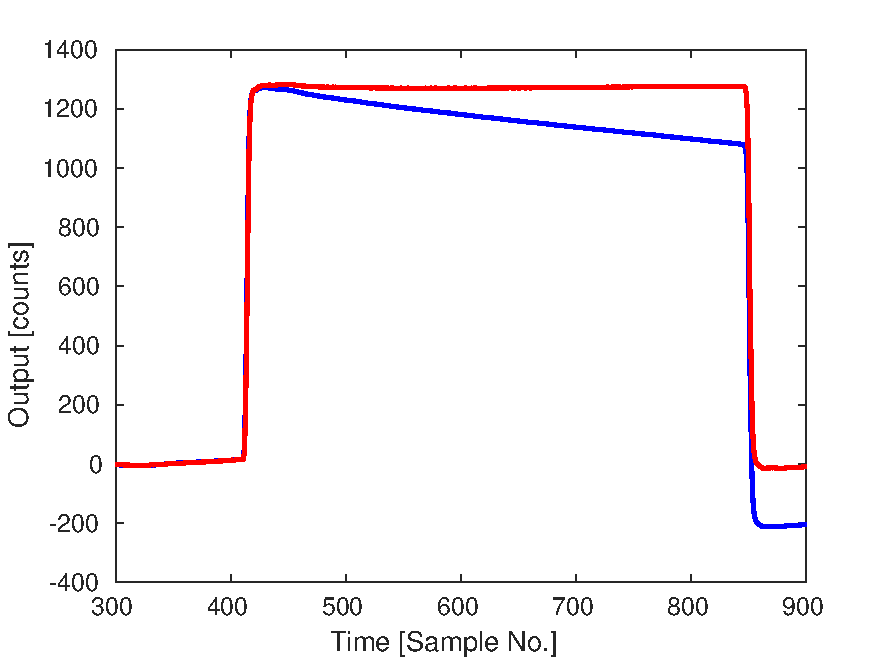
\includegraphics[width=0.8\textwidth]{Figures/commissioning/iirDiodeFiltOffOn}
  \caption{Diode output on the FONT5a board with the IIR filter off (blue) and on (red).}
  \label{f:iirDiodefiltOffOn}
\end{figure}

The droop emerges as a result of the use of AC coupling on the ADC input transformers for electrical isolation. This involves using a capacitor, the current across which is dependent on \({dV}/{dt}\) (\(V\) being voltage and \(t\) time), to remove the DC component (or mean offset) from a signal \cite{acCoupling}. In particular for the diode channel the output is increasingly well described by a DC signal on the flat top as you move away from the leading edge of the pulse, with the capacitor causing droop in the response as a result. There is also a small effect on the mixer output, as will be seen later.

In the simplest case the droop should be well described by an exponential decay of the form \(A\exp\left(-t/\tau\right)\), where \(t\) is the time or sample number along the pulse and \(\tau\) is the decay time constant. For the FONT5 board this only gave a rough approximation of the true droop characteristics due to non-linear properties of the input transformers. On the updated FONT5a board the transformers were changed to both reduce the magnitude of the droop and give closer to the expected exponential decay \cite{colinPriv}. Figure~\ref{f:iirDiodeFit} shows an exponential fit to the Mon1 diode output as seen on the FONT5a board (ADC1). Apart from a small deviation at the beginning of the pulse the agreement is excellent, with residuals to the fit of only up to 2~counts compared to a signal magnitude of 1250~counts. For ADC1 the fitted decay time constant is \(\tau = 838\pm16\)~samples, or \(2.35\pm0.05~\mathrm{\mu}\)s (with one ADC sample every 2.8~ns at 357~MHz). Each ADC on the FONT5a board has slightly different droop characteristics, with the decay time constant for ADC2 being \(938\pm18\)~samples, for example (calculated with the diode moved on to ADC2).

\begin{figure}
  \centering
  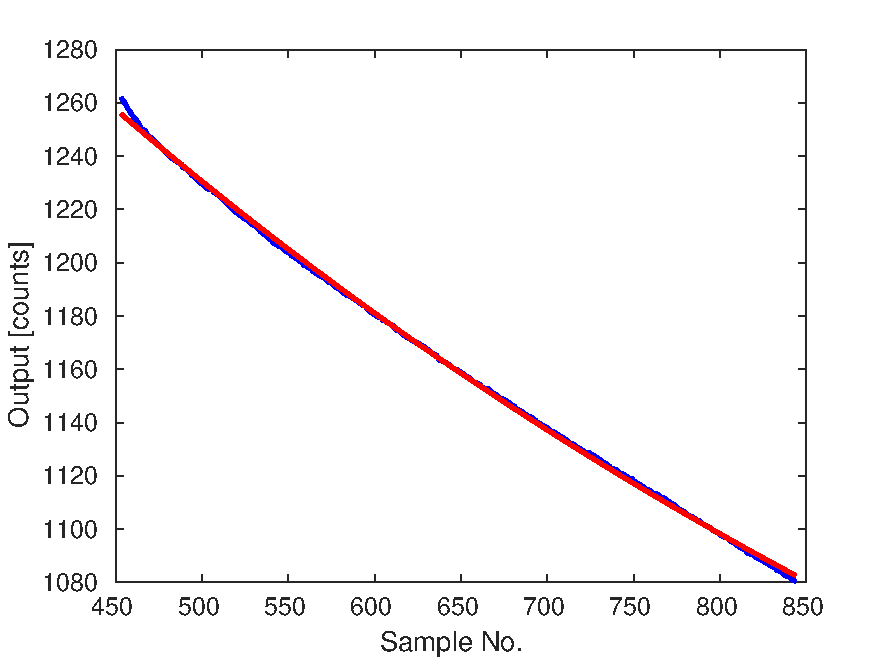
\includegraphics[width=0.8\textwidth]{Figures/commissioning/iirDiodeFit}
  \caption{Exponential fit (red) to droop on the measured diode output (blue).}
  \label{f:iirDiodeFit}
\end{figure}

\begin{figure}
  \centering
  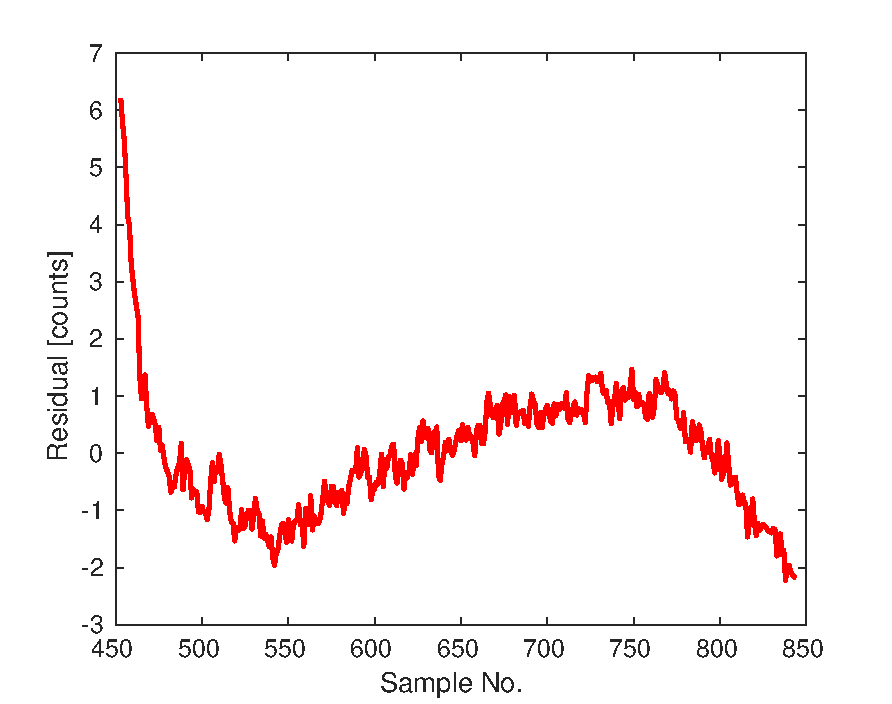
\includegraphics[width=0.8\textwidth]{Figures/commissioning/iirDiodeFitResid}
  \caption{Residuals between the measured diode output and the exponential fit to the droop shown in Figure~\ref{f:iirDiodeFit}.}
  \label{f:iirDiodeFitResid}
\end{figure}

In the case where the diode is used in the phase reconstruction as originally envisaged the ADC droop would propagate in to the applied correction and create an output to the amplifier that increases with time with respect to the ideal value (as the Mixer is divided by sqrt(Diode)). The effect on the correction is much smaller without diode normalisation but it still slightly distorts the measured Mixer input to ADC2. Therefore, a digital Infinite Impulse Response (IIR) filter has been implemented in the FONT5a board firmware to remove the exponential droop in the ADC outputs \cite{glennCLIC14}. This works by recursively adding the expected droop to the ADC output based on the known decay constants, so that:
\begin{equation}
y(t) = x(t) + \frac{1}{\tau} \sum_{i=1}^{t} x(i-1)
\end{equation}
\label{e:iirFilt}
Here \(y(t)\) is the filtered ADC output at sample \(t\), \(x(t)\) is the original unfiltered output at sample \(t\), and \(\tau\) is the decay time constant. Rather than being hard-coded in the firmware the applied decay constant in the filter for each ADC is calculated using an 8-bit \(\pm64\) filter weight (set in the DAQ), which is then divided by a common division factor to get the real applied value of \(1/\tau\) \cite{glennPriv}. The optimal filter weights for each ADC in the FONT5a board currently used for PFF operation are shown in Table~\ref{t:filtWeights}, these can be converted in to the true decay constant values using the fitted values for ADC1 and ADC2 quoted above.

\begin{table}
  \begin{center}
    \begin{tabular}{| c | c |}
	   \hline
       ADC & Filter Weight \\ \hline
       1 (Mon1 Diode) & 50 \\
	   2 (Mon1 Mixer) & 56 \\
	   3 & 50 \\
	   4 & 53 \\
	   5 & 45 \\
	   6 & 51 \\
	   7 & 48 \\
	   8 & 55 \\
	   9 & 49 \\
 	   \hline
    \end{tabular}
    \caption{Fitted IIR filter weights for the FONT5a board ADCs.}
  	\label{t:filtWeights}
  \end{center}
\end{table}

With the IIR filters enabled on the FONT5a board the droop on the diode (ADC1) is almost perfectly removed as shown in Figures~\ref{f:iirDiodefiltOffOn}~and~\ref{f:iirDiodefiltOffOn_zoom}, although in the zoomed in figure some slight deviation from flat is visible due to the residuals around the exponential fit seen previously. The effect on the reconstructed phase using only the mixer (ADC2) is shown in Figure~\ref{f:iirPhasefiltOffOn}, with a modest adjustment to the overall shape that is most visible at the start and end of the pulse.

\begin{figure}
  \centering
  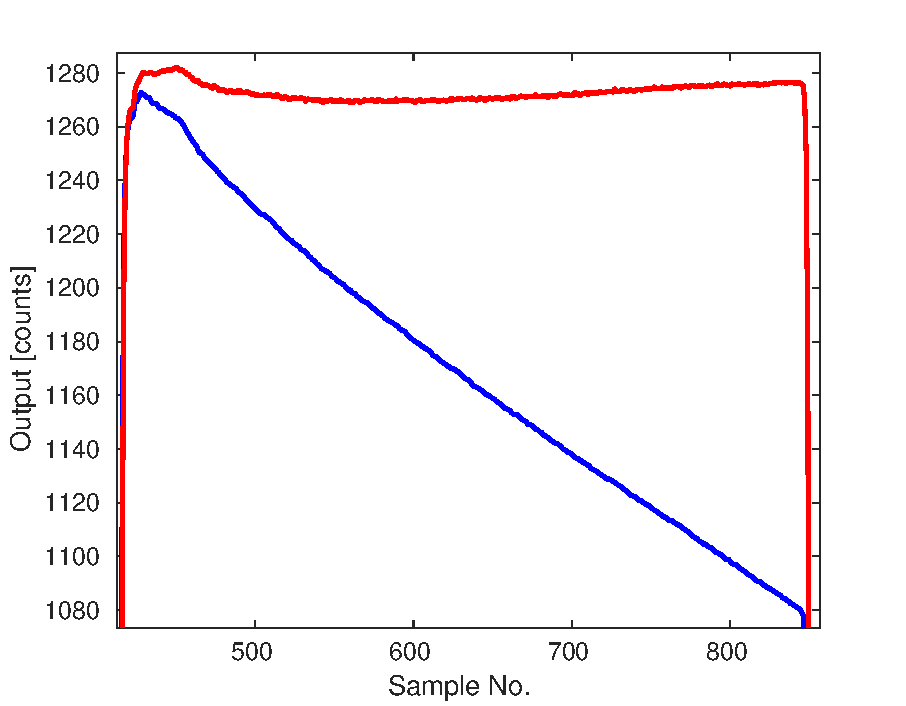
\includegraphics[width=0.8\textwidth]{Figures/commissioning/iirDiodeFiltOffOn_zoom}
  \caption{Meausred diode output on the FONT5a board with the IIR filter off (blue) and on (red). Zoomed in to show deviations from the ideal square wave that are not visible in Figure~\ref{f:iirDiodefiltOffOn}.}
  \label{f:iirDiodefiltOffOn_zoom}
\end{figure}

\begin{figure}
  \centering
  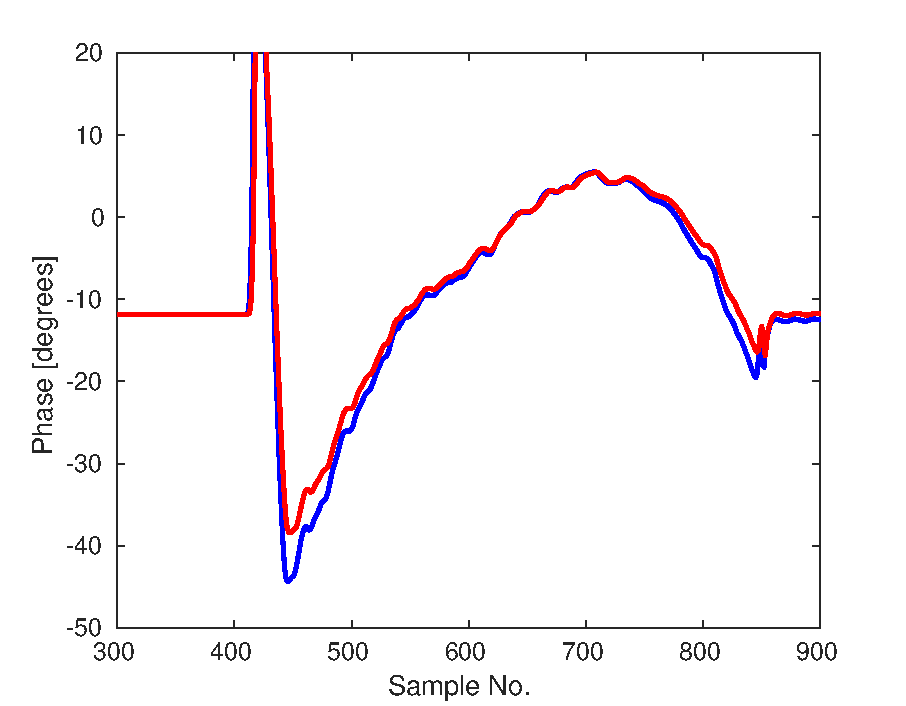
\includegraphics[width=0.8\textwidth]{Figures/commissioning/iirPhaseFiltOffOn}
  \caption{Meausred phase on the FONT5a board with the IIR filter off (blue) and on (red).}
  \label{f:iirPhasefiltOffOn}
\end{figure}


\subsection{Gain Calculation}
\label{ss:fontGain}

As shown in Section~\ref{s:pffEquations} the effect of the PFF system can be modelled by simply subtracting the measured upstream phase, \(\phi_u\), from the downstream phase, \(\phi_d\) with a gain factor, \(g\):
\begin{equation} \label{e:realGainEqn}
\phi_{PFF} = \phi_d - g\phi_u
\end{equation}
Here \(\phi_{PFF}\) is the corrected downstream phase. The gain set in the FONT5a DAQ is not directly a multiplication factor in terms of the phase, but rather a multiplication in terms of DAC counts and other constants. How the set gain on the FONT5a board relates to the true gain \(g\) is derived in this section.

In the case where diode normalisation is not used, which is the nominal setup, the DAC outputs when the PFF system is enabled are given by:
\begin{eqnarray}
\mathrm{DAC1} = \frac{\mathrm{F1}}{64}\mathrm{ADC2} \nonumber \\ 
\mathrm{DAC2} = \frac{\mathrm{F2}}{64}\mathrm{ADC2} \label{e:fontGain1}
\end{eqnarray}
Here \(\mathrm{DAC1}\) and \(\mathrm{DAC2}\) are the two DAC outputs, in DAC counts, \(\mathrm{F1}\) and \(\mathrm{F2}\) are the respective gains for each DAC output set in the DAQ, and \(\mathrm{ADC2}\) is the Mon1 mixer signal level in ADC counts, which is connected to ADC2 for normal PFF operation. The whole calculation uses 16-bit architecture, with the 3 sub-integer bits discarded when sent to the 13-bit DACs \cite{glennPriv}. The FONT gains \(\mathrm{F1}\) and \(\mathrm{F2}\) are 14-bit (\(\pm8192\)) and the common division factor of \(1/64\) is set by several parameters fixed in the FONT5a firmware in order to give a sensible range of gain values based on the approximate signal levels \cite{glennPriv}. Typically \(\mathrm{F2} = -\mathrm{F1}\), so that the beam is deflected in opposite directions in each kicker to achieve orbit closure in the chicane. With a maximum gain of 8192 an ADC2 input of 1~ADC~count gives an output of 128~DAC~counts. If diode normalisation is enabled the expressions above are multiplied by \(1/\sqrt{\mathrm{ADC1}}\) (with the Mon1 diode signal connected to ADC1 in normal operation) and different scale factors are used \cite{glennPriv}.

To determine the optimal values for F1 and F2 given the current beam conditions it is important to know how they translate in to the real applied gain \(g\) from Equation~\ref{e:realGainEqn}. The real gain \(g\) is related to the DAC outputs derived above by:
\begin{equation} \label{e:fontGain2}
g\phi_u = k\mathrm{DAC}
\end{equation}
Where \(k\) is the phase shift, in radians, in the chicane resulting from a DAC output of 1 count. The indices 1 and 2 are dropped from \(\mathrm{DAC1,~DAC2,~F1}\) and \(\mathrm{F2}\) from this point for simplicity. The upstream phase, also in radians, can then be related to the ADC2 input by:
\begin{equation} \label{e:fontGain3}
\phi_u \simeq \frac{\mathrm{ADC2}}{A}
\end{equation}
Here \(A\) is the calibrated maximum Mon1 mixer amplitude, in ADC counts, determined in the same way as Section~\ref{s:monCalibrations}. Note that both this and the direct proportionality with ADC2 in Equations~\ref{e:fontGain1} assume the small angle approximation \(\mathrm{ADC2} = A\sin\phi_u \simeq A\phi_u\) for small \(\phi_u\). This is done for latency reasons \cite{glennPriv} and its effect on the accuracy of the applied correction is discussed in Section~\ref{ss:fontSmallAng}.

Combining Equations~\ref{e:fontGain1},~\ref{e:fontGain2}~and~\ref{e:fontGain3} gives:
\begin{align}
\frac{g}{A}\mathrm{ADC2} &= \frac{k\mathrm{F}}{64}\mathrm{ADC2} \nonumber \\
g &= \frac{kA}{64}\mathrm{F} \label{e:fontGain4}
\end{align}
In Section~\ref{ss:corrRange} a phase shift of \(3.5^\circ\) per volt sent to the amplifier is determined. Knowing that 4096 DAC counts corresponds to 2~V sent to the amplifier this value can be converted into \(k = 29.8~\mathrm{\mu}\)radians/DAC~count. Typical calibrations for Mon1 on the FONT5a board give \(A \simeq 3440\)~ADC~counts (Section~\ref{ss:FONTCal}). Overall, the actual effective gain therefore relates to the gain as set in the DAQ via:
\begin{equation}
g \simeq \frac{\mathrm{F}}{624}
\end{equation}
The optimal gain to apply (Section~\ref{s:pffEquations}) is given by the upstream-downstream phase correlation, \(\rho_{ud}\), multiplied by the downstream-upstream jitter ratio, \(\sigma_{d}/\sigma_{u}\):
\begin{equation}
g_{\mathrm{opt}} = \frac{\sigma_{d}}{\sigma_{u}} \rho_{ud}  
\end{equation}
Therefore the optimal gain to set in the units used in the DAQ, dependent on the current beam conditions, is:
\begin{equation}
F_{\mathrm{opt}} \simeq 624 \frac{\sigma_{d}}{\sigma_{u}} \rho
\label{e:fontOptGain}
\end{equation}
In good conditions the correlation and jitter ratio are close to one, although the downstream phase jitter can be up to a factor two larger than the upstream jtiter at CTF3 thus the applied gains in the DAQ are typically in the range between 625 and 1250.

\subsection{Effect of Using Small Angle Approximation}
\label{ss:fontSmallAng}

As mentioned previously the phase calculation in the PFF algorithm in the FONT5a firmware uses the small-angle approximation, thus differs from the correct full phase reconstruction method used in Chapter~\ref{c:phaseMons} as follows:
\begin{align}
\phi_{\mathrm{SA}} &= \frac{\mathrm{Mixer}}{A} \\
\phi_{\mathrm{FULL}} &= \arcsin\left(\frac{\mathrm{Mixer}-d}{A}\right)
\end{align}
Where \(\phi_{\mathrm{SA}}\) and \(\phi_{\mathrm{FULL}}\) are the upstream phase calculated using the small angle approximation
and with the full phase reconstruction method respectively. \(\mathrm{Mixer}\) is the phase monitor mixer output, \(A\) is the phase monitor calibration amplitude and \(d\) is the calibration offset needed to take in to account asymmetry in the mixer minimum and maximum output due to cross-talk from the diode (Section~\ref{ss:sigGenDiode}).
The PFF correction output is \(\phi_{\mathrm{SA}}\), using the upstream 
phase monitor Mon~1, multiplied by a gain factor.

Any differences between the calculated phase with the small angle
approximation and the actual phase using the full phase reconstruction
 method will lead to imperfections in the applied PFF correction.
The calculated phase with each approach is plotted in Figure~\ref{f:phaseRecDiff} for offsets between the beam phase and the electronics LO phase between \(\pm90^\circ\). For small incoming phases (close to zero Mixer output) the only difference between the two methods is a static offset of \(-d/A\) in the measured phase, and this holds up to \(\pm10^\circ\) (and is a good approximation up to \(\pm20^\circ\)). In this case the applied correction will also contain this constant offset, but the corrected downstream phase jitter, which has been the only focus of the PFF prototype to date, will still be optimal. 

With larger offsets between the beam phase and the LO (large Mixer output) the small angle approximation is no longer valid and the difference between the two methods rises to up to \(35^\circ\). Most importantly the measured phase, and therefore the correction output, is no longer linearly dependent on the incoming beam phase when there is a large offset between the beam and LO phases. In the most extreme case, the measured phase difference between two pulses with a beam-LO phase offset of \(80^\circ\) and \(90^\circ\) would only be \(1^\circ\) when using the small angle approximation, instead of the expected \(10^\circ\). In turn, the difference in the correction applied to the two pulses would only be \(1^\circ\) instead of \(10^\circ\), degrading the achievable corrected phase jitter.

\begin{figure}
  \centering
  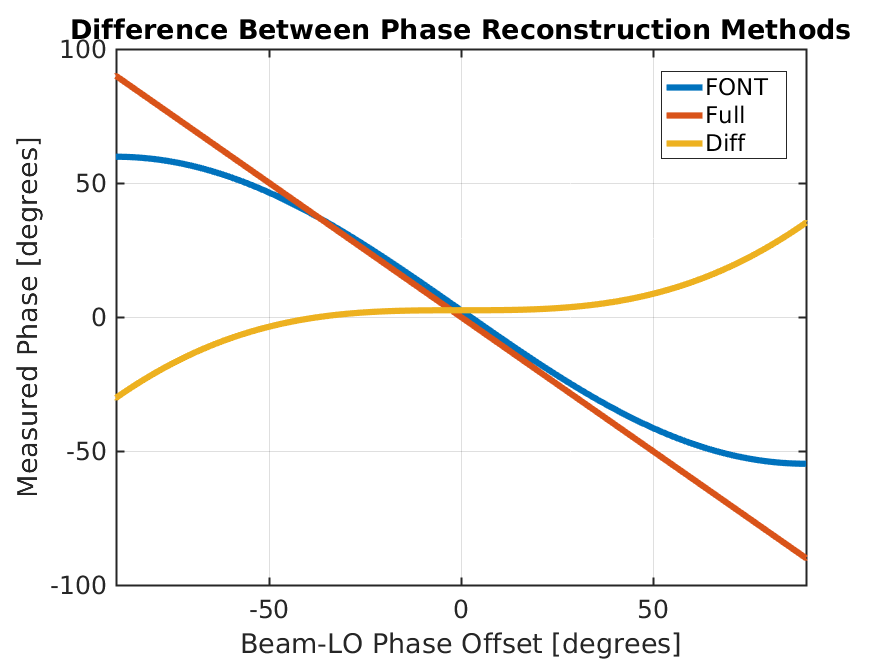
\includegraphics[width=0.8\textwidth]{Figures/commissioning/phaseRecDiff}
  \caption{Difference (green) between a phase reconstruction method using the small angle approximation (blue), and the full reconstruction method taking in to account non-linearities in the mixer output for large phase offsets (red).}
  \label{f:phaseRecDiff}
  \centering
  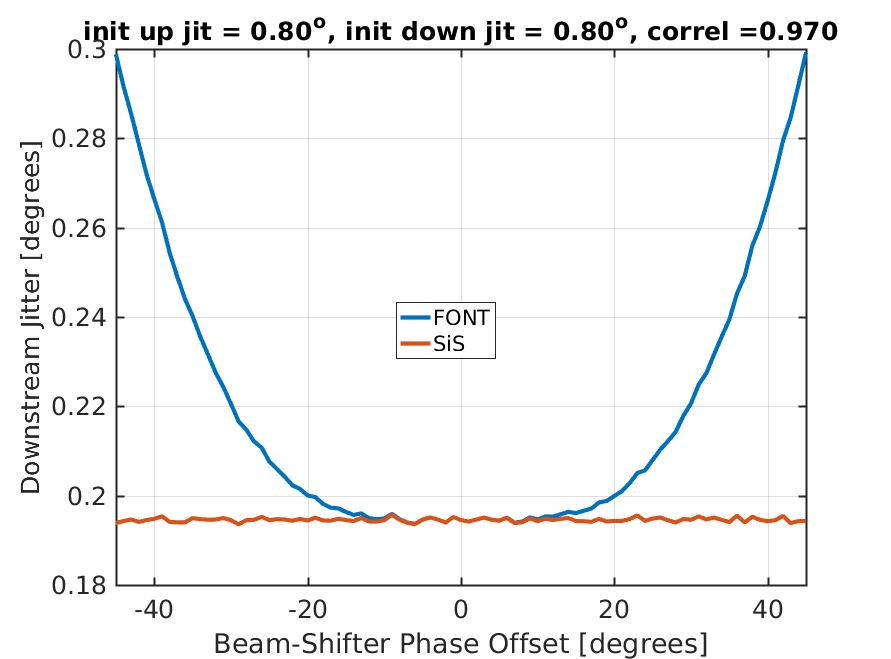
\includegraphics[width=0.8\textwidth]{Figures/commissioning/phaseRecJitSim}
  \caption{Achievable PFF jitter versus phase offset for the full phase reconstruction method (red), and the phase reconstruction using the small angle approximation (blue).}
  \label{f:phaseRecJitSim}
\end{figure}

Figure~\ref{f:phaseRecJitSim} shows a simulation of the theoretical downstream jitter that can be achieved with both phase reconstruction methods with \(0.8^\circ\) initial upstream and downstream phase jitter and an upstream-downstream phase correlation of \(97\%\). These values are chosen to represent the beam conditions that will need to be achieved in order to demonstrate \(0.2^\circ\) phase stability at CTF3. In the \(\pm10^\circ\) region where the small approximation holds there is no degradation in the achievable corrected phase jitter using the simplified method in the PFF algorithm. Outside this region the jitter is degraded, increasing from below \(0.2^\circ\) to \(0.3^\circ\) for a beam-LO phase offset of \(50^\circ\). 

As the correction range of the PFF system is less than \(\pm10^\circ\) (Section~\ref{ss:corrRange}) there should be no degradation in the PFF performance resulting from the use of the small angle approximation in the PFF algorithm, providing the LO phase shifter in the phase monitor electronics has been set correctly. This highlights the importance to adjust the phase shifters to zero the Mixer output not only in order to maximise the phase monitor resolution (Section~\ref{ss:resVsShifter}) but also to ensure the correction calculation itself is valid. However, it is perhaps interesting to note that it would not be possible to correct the full CTF3 pulse length to \(0.2^\circ\) jitter with this implementation of the PFF algorithm even if the correction range were large enough to encompass the \(40^\circ\) phase sag.

\newsection{amplifierSetup}{Amplifier}

The amplifier takes the two DAC signals from the FONT5a board and
uses them to produce four high voltage outputs. These are connected to the downstream ends of the kicker strips (two kickers and two strips per kicker gives four connections at the downstream ends in total), creating the potential difference between the strips that deflects the beam in order to correct the phase. The returning signals from the upstream ends of the kicker strips are then terminated back at the amplifier. As the amplifier is installed together with the phase monitor electronics and FONT5a board in the klystron gallery the cables between the amplifier and kickers are long and represent the single largest contribution to the overall system latency, as discussed in Section~\ref{ss:kickerCables}. This section discusses the design and performance aspects of the amplifier that are relevant to PFF operation.

\subsection{Design}
\label{ss:ampDesign}

The amplifier is purpose built for the PFF prototype, also by the FONT group at Oxford University, with further details of its design available in \cite{colinCLIC16}. An annotated picture of its front panel is shown in Figure~\ref{f:AmplifierPanelPic} and a smplified diagram showing the flow of signals between the FONT5a board, amplifier and kickers is shown in Figure~\ref{f:amplifierDiagram}.
The amplifier is installed in a standard 3U rack and has a modular design. It consists of five individual modules split between two sides, labelled left and right. The left side of the amplifier, which uses the DAC~1 output, powers the first kicker in the chicane, and the right side of the amplifier, which uses the DAC~2 output, powers the second kicker. Each side of the amplifier contains its own ``drive module'' and ``terminator module''. Finally there is a central ``control module'' that is common to both sides of the amplifier.

All the outputs from the FONT5a board are connected to the control module, this includes the DAC~1 and DAC~2 outputs as well as the trigger for the amplifier. The required 24~V, 1.1~A power supply is also connected to the control module. The control module then deals with the distribution of power, timing and input signals (derived from the DAC inputs) to the two drive modules. The control panel can therefore include signal processing designed to protect the drive modules. It ensures the maximum signal level sent to the drive modules is at a safe level and limits the rate of large changes in the input drive signal (limits the slew-rate), as well as preventing triggering of the drive modules if a problem is detected, for example.

The amplification of the signals to create the high voltage outputs occurs in the drive modules. Each drive module takes one input signal but creates two high voltage outputs (A and B) which have equal magnitude but opposite polarity. These are connected to the downstream end of the left and right strips of one of the kickers, to create a potential difference across the kicker strips that is double the voltage of each individual drive output. The signal amplification consists of low voltage Si FETs (Ixys DE150-201N09A \cite{ixysFET}) driving high voltage SiC FETs (Wolfspeed C2M0160120D \cite{wolfFET}) and a final output transformer, giving a peak output of around \(\pm700\)~V (seen in more detail in Section~\ref{ss:ampLin}). The output has a bandwidth of 47~MHz for small signal variations up to 20\% of maximum output (around 140~V). The bandwidth for larger variations is slew rate limited, and around 25~MHz for variations up to 50\% of the maximum output, for example \cite{colinCLIC16}.

Each drive module requires a ramp up time of 1~\(\mathrm{\mu s}\), which defines when the trigger must arrive from the FONT5a board. After this period the drive modules are powered for 1.6~\(\mathrm{\mu s}\)  with full output across 1.3~\(\mathrm{\mu s}\) (slightly longer than needed to correct the full 1.1~\(\mathrm{\mu s}\) CTF3 beam pulse length). The control module includes a monitoring output (labelled ``ON'') that can be digitised to observe the time period within which the drive modules are on and ready to receive input.

The high voltage signals leaving the upstream ends of the kicker strips are terminated back at the amplifier on the terminator modules. Each module consists of two 50~\(\mathrm{\Omega}\) terminators designed to be able to withstand the maximum 20~kW output from the drive modules \cite{colinCLIC16}. Each terminator has a monitoring signal, which gives output at around -40~dB or approximately 1/115 of the input voltage \cite{colinPriv}. These can be used to verify the applied output from the drive modules is as expected, and form the basis of most of the measurements in the remainder of this section as well as the timing checks in Section~\ref{ss:absTiming}, for example.

The description of the amplifier here represents the version of the amplifier that was used for the latest PFF tests, and for almost all results in this thesis. A first version of the amplifier, with around half the output voltage at up to \(\pm350\)~V was used for early PFF tests. Additional FETs were added in the second version described above to boost the output voltage to \(\pm700\)~V. A third version of the amplifier was forseen but ultimately deemed unnecessary for the application at CTF3. This would have provided a voltage of up to \(\pm1400\)~V by combining the output of four individual drive modules \cite{glennCLIC13}.

\afterpage{\begin{landscape}
\begin{figure}
  \centering
  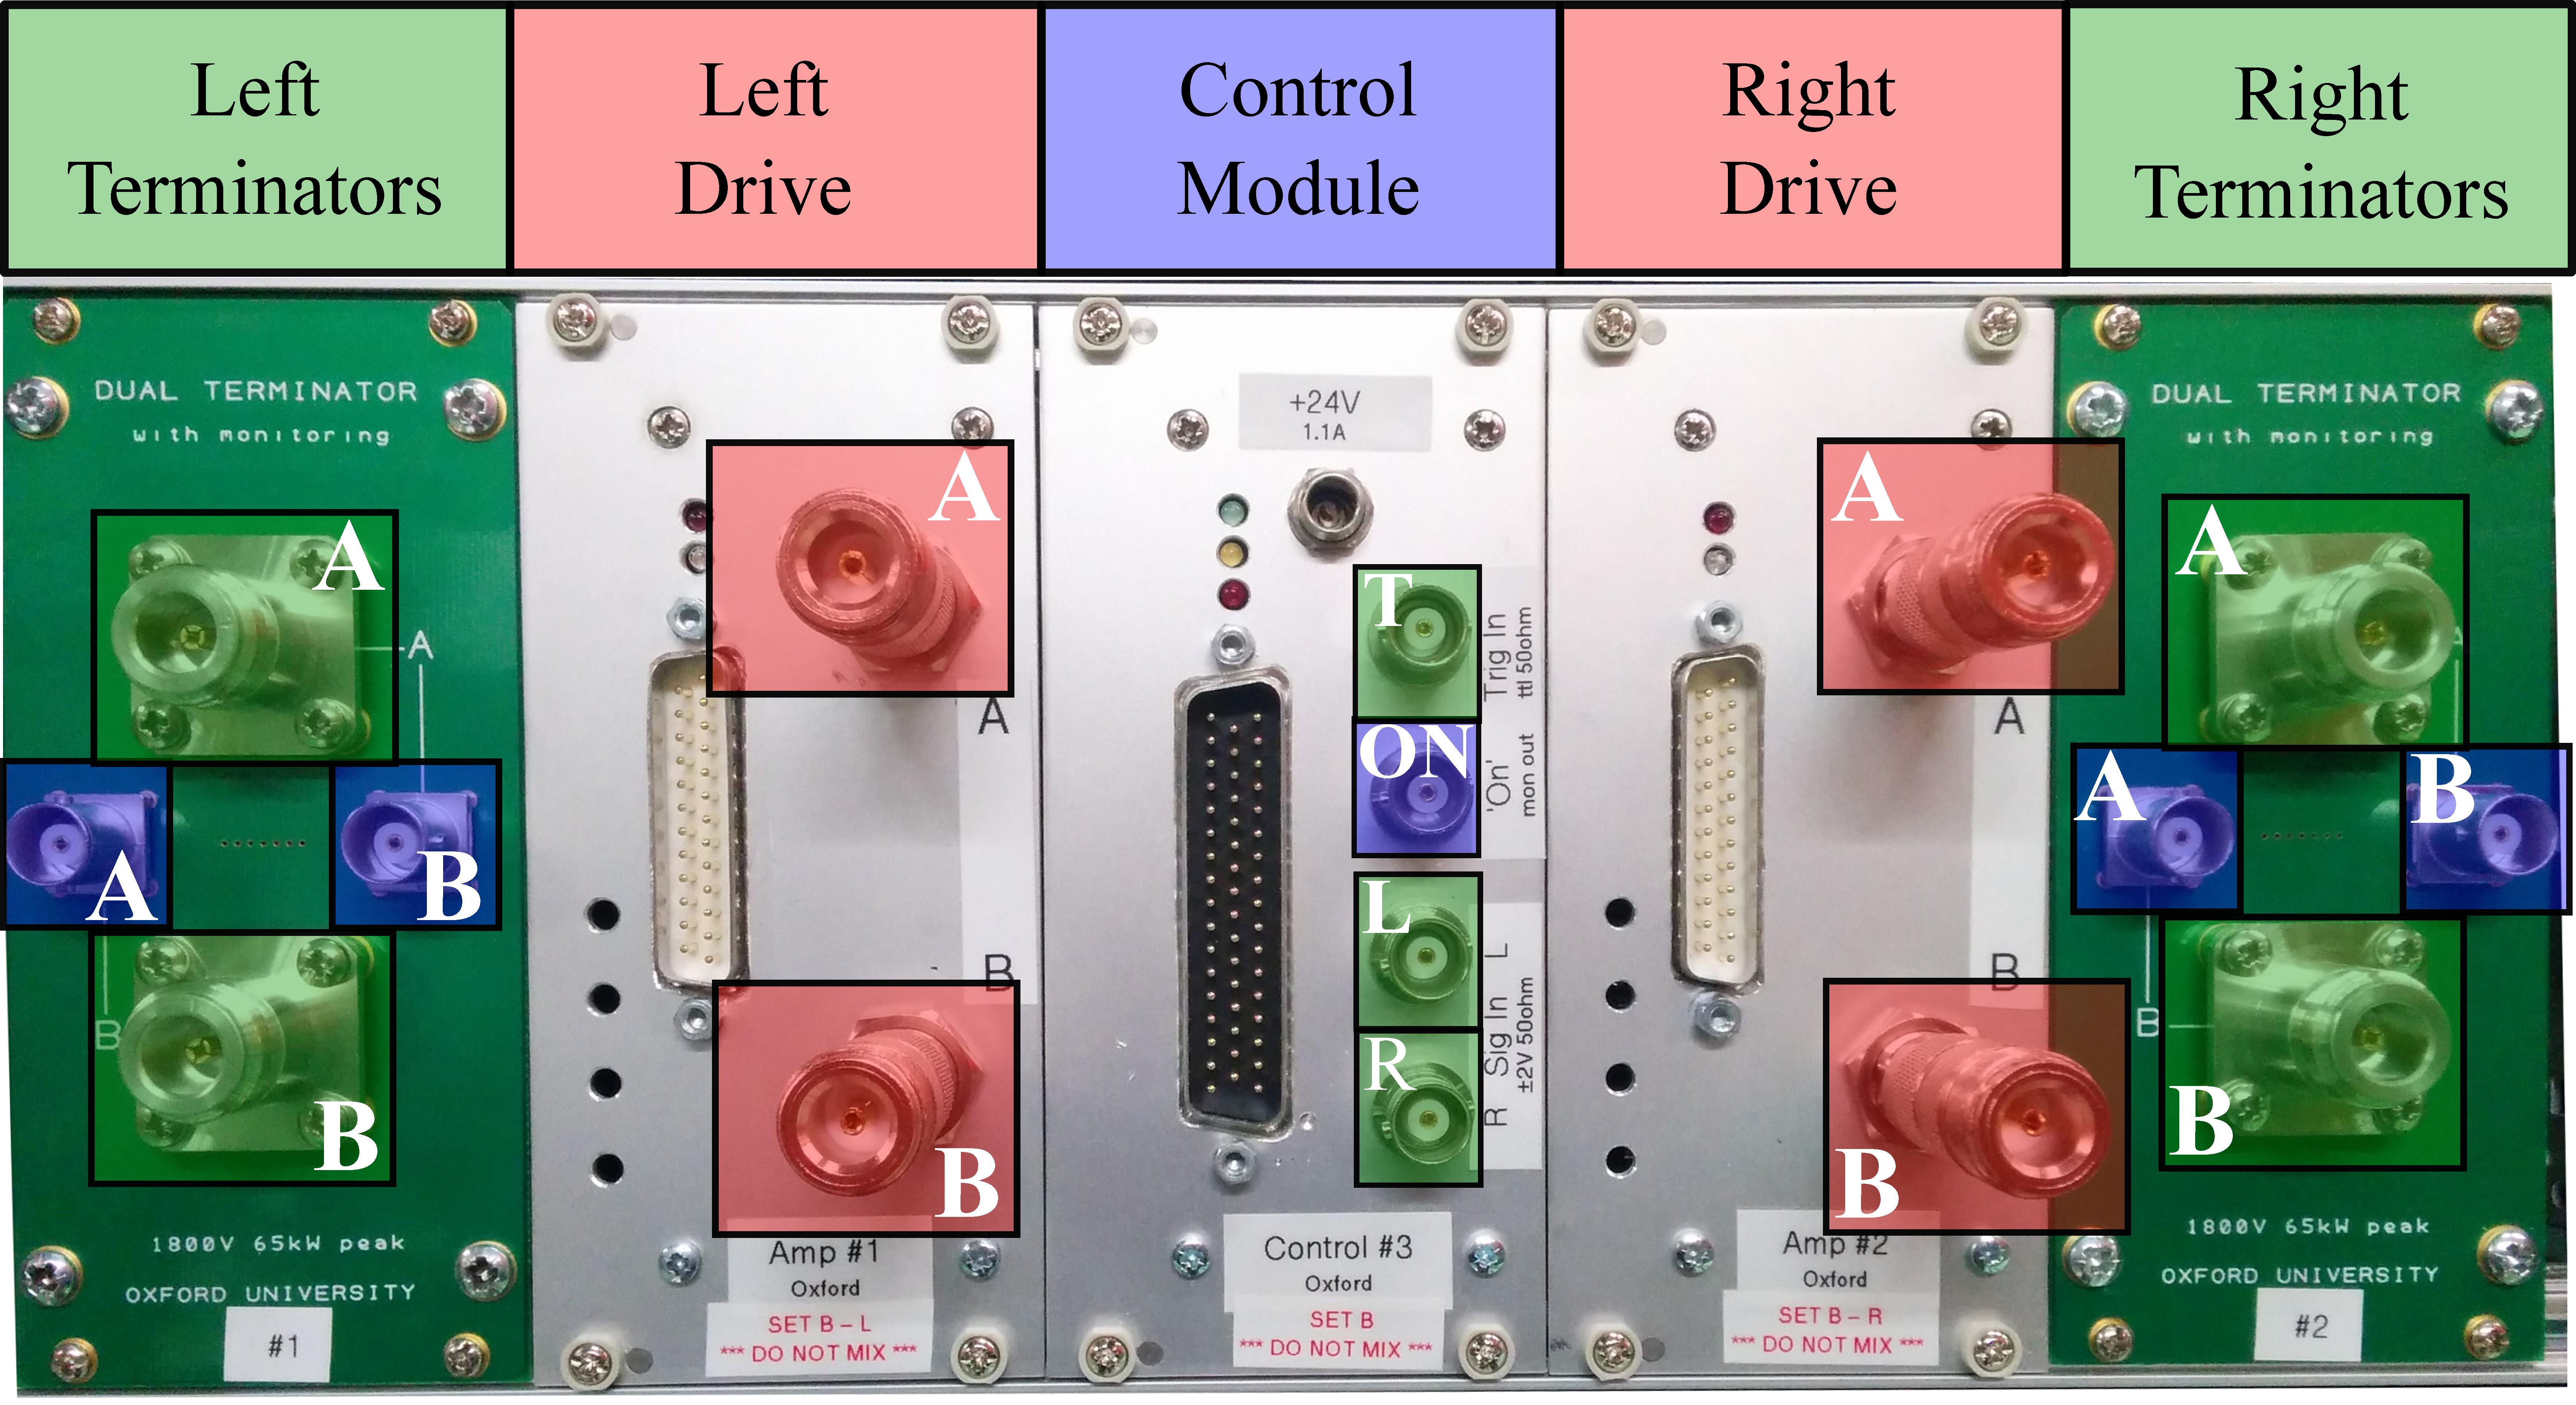
\includegraphics[width=0.9\hsize]{Figures/commissioning/AmplifierPanelPic}
  \caption{Front panel of the amplifier. Inputs to the amplifier are highlighted in green, drive outputs in red and monitoring outputs in blue. Inputs to the control module are the trigger (T) and the two DAC outputs from the FONT5a board used to determine the drive to the left (L) and right (R) sides. Each side of the amplifier has two pairs of drive outputs and terminators, A and B. The signal returning to each of the terminators can be observed on their corresponding monitoring outputs. The monitoring output on the control module (ON) shows the 1.4~\(\mathrm{\mu}\)s time during which the amplifiers are able to provide their output. Not highlighted in the figure are the 24~V, 1.1~A power connector at the top of the control module, and also the three custom connectors used to communicate between the control module and drive modules.}
  \label{f:AmplifierPanelPic}
\end{figure}
\end{landscape}}

\afterpage{\begin{landscape}
\begin{figure}
  \centering
  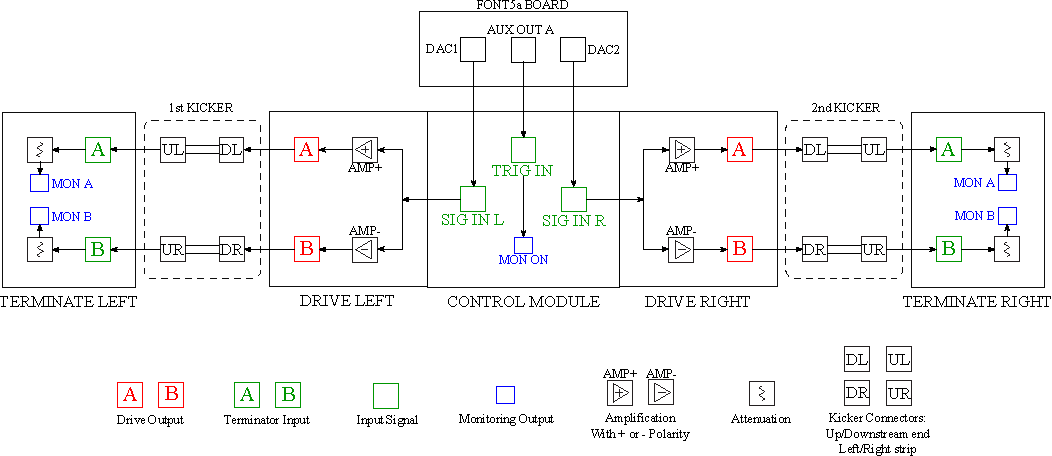
\includegraphics[width=\hsize]{Figures/commissioning/amplifierDiagram}
  \caption{Simplified flow diagram showing the connections between the FONT5a board, the amplifier and the kickers. The kickers are inserted between the drive and terminator modules for the purposes of the diagram, but in reality the terminator modules neighbour the drive modules in the same unit as seen in Figure~\ref{f:AmplifierPanelPic}. Note that the A and B outputs on each side always have opposite polarity, as needed to create a large potential difference between the kicker strips.}
  \label{f:amplifierDiagram}
\end{figure}
\end{landscape}}

\subsection{Linearity}
\label{ss:ampLin}

Figure \ref{f:AmpOutvsDAC} shows the amplifier output, as measured by the monitoring signals, at different constant input voltages sent from the FONT5a board between the minimum of -2V (-4095 DAC counts) and maximum of 2V (+4095 DAC counts). The output voltage from the monitoring signals is converted in to the real amplifier output Voltage using the approximate conversion factor of 115. All four amplifier outputs are shown (one for each strip of the two kickers). The plotted values are means taken across a 480~ns central part of the whole 1400~ns output pulse.

The relative polarity of the four outputs used is equivalent to what would be applied to the kickers during PFF operation, with opposite polarity of the L and R amplifier outputs (powering the first and second kicker respecitvely), so that the beam is kicked in opposite directions by each kicker. The second kicker should then act to close the orbit bump created by the first kicker. Within each side of the amplifier the A and B outputs (applied to the left and right strip of each kicker respectively) also have opposite polarity. This is necessary to create the potential difference between the kicker strips that produces the deflecting field for the beam. The relative polarity of the A and B outputs is fixed in the amplifier design and cannot be controlled via the FONT5a board.

The response of the amplifier is highly linear in the region between \(\pm1.2\)~V sent to the amplifier. Outside this range the amplifier clearly begins to enter saturation, in particular above input voltages of \(\pm1.7\)~V. The linear fits shown include only the points between \(\pm1.2\)~V, excluding the first and last three points in the scan of input voltages, in order to not be biased by the effects of saturation.

Figure \ref{f:AmpOutvsDAC_residual} shows the residuals between the linear fit and the real amplifier output across the full range of input voltages. By looking at the residuals a slight deviation from linearity in the \(\pm1.2\)~V range is also visible, although the maximum difference is only 10~V or a 3\% relative error. At the maximum input voltage of \(\pm2\)~V the difference between the real output and the amplitude expected if the response was linear across the full range rises above 150~V, or a relative error of more than 25\%. For example, the RB output at an input voltage of \(+2\)~V is 605~V but the fitted response gives 769~V, a difference of 164~V or 27\%.

The effects of amplifier saturation are not taken in to account in the PFF algorithm on the FONT5a board, in which the DAC output is linearly dependent on the input phase (voltage from the phase monitor mixer signal) across the full range. The applied correction to the downstream phase will therefore be non-optimal when the DAC output calculated by the PFF algorithm is above an absolute value of 2500 counts (1.2~V sent to the amplifier). To date the non-linearity of the amplifier as it begins to enter saturation has also not been included in the PFF simulations presented in the following chapters. This may partially explain the small discrepancies seen between the simulated and real results in some datasets, so including the effect will be pursued in the future. In addition, it could be foreseen to incorporate the saturation characteristics in to the PFF algorithm on the FONT5a board, so that calculated outputs above 2500 counts are boosted slightly to compensate for the lower than expected amplifier output.

Discrepancies between the four amplifier outputs are also visible in Figure~\ref{f:AmpOutvsDAC_residual} and Table~\ref{t:AmpOutVsDAC}, both in terms of gradient and peak output. This can be partially but not completely explained by errors of up to a few percent in the precise calibration of the four monitoring outputs, which do not output exactly 1/115 of the real input voltage \cite{colinPriv}. Differences between the A and B outputs sent to each kicker are not an issue for the PFF performance as both are linear (in the \(\pm1.2\)~V range) and the kick experienced by the beam in each kicker is proportional to the difference of the two. Therefore, only the calibration between the output from the FONT5a board sent to the amplifier and the resulting phase shift in the TL2 chicane is affected. However, disparity between the potential difference across each kicker (LA-LB and RA-RB), so that the deflection of the beam in each kicker is different, leads to the orbit bump created by the PFF system not being closed in the chicane, degrading the horizontal beam stability downstream. The fitted potential difference at 1~V input is 869~V for the left amplifier (LA-LB, sent to the first kicker) and 835~V for the right amplifier (RA-RB, sent to the second kicker), a difference of 4\%. This could be compensated in the PFF setup on the FONT5a board by using a different gain for each correction output, so that the DAC output to the right amplifier is higher but the resulting voltage applied to both kickers is the same. Orbit closure is discussed further in Section~\ref{ss:orbitClosure}.


\begin{figure}
  \centering
  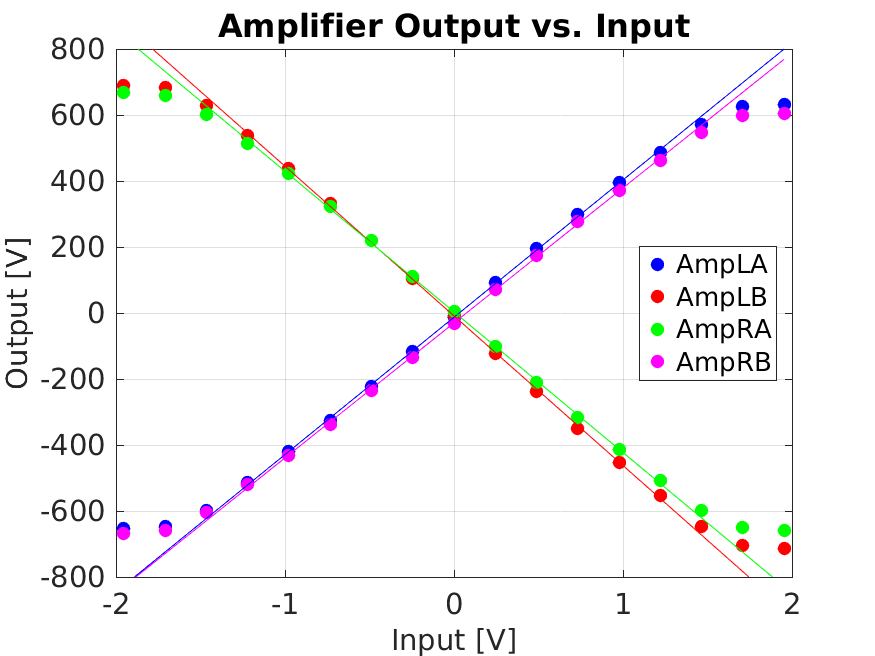
\includegraphics[width=0.8\textwidth]{Figures/commissioning/AmpOutvsDAC}
  \caption{Mean output of each amplifier channel vs. the input voltage. The four amplifier channels are: LA (blue), LB (red), RA (green) and RB (magenta). Markers show the measured output, and lines a linear fit to the output in the \(\pm1.2\)~V input range.}
  \label{f:AmpOutvsDAC}
  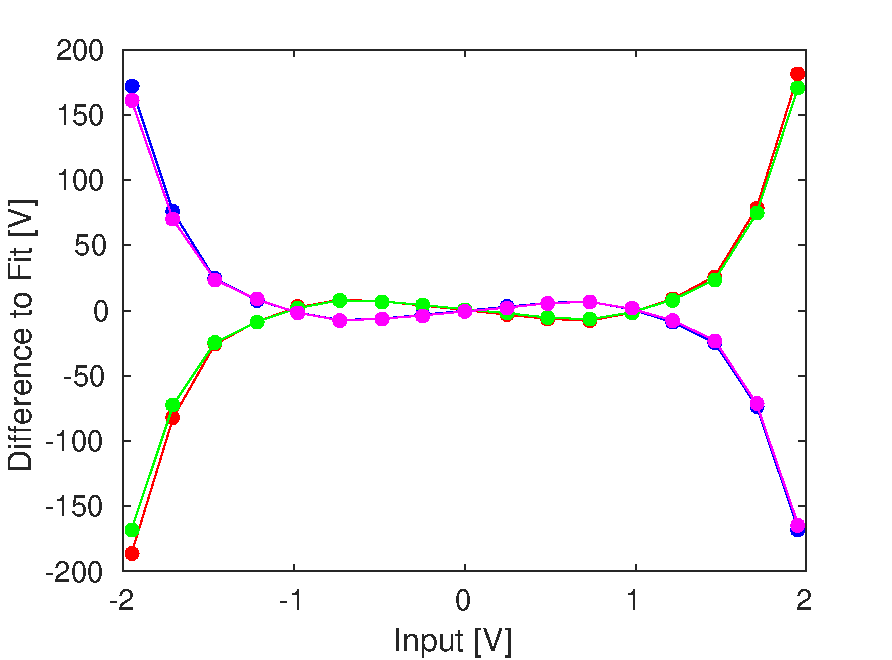
\includegraphics[width=0.8\textwidth]{Figures/commissioning/AmpOutvsDAC_residual}
  \caption{Residuals between the amplifier output voltage and the linear fits seen in Figure~\ref{f:AmpOutvsDAC}. The four amplifier channels are: LA (blue), LB (red), RA (green) and RB (magenta). }
  \label{f:AmpOutvsDAC_residual}
\end{figure}

\begin{table}
  \begin{center}
    \begin{tabular}{| c c c |}
	   \hline
       Amplifier Port & Input Voltage & Output Voltage \\ \hline
       LA & +1~V & \(+416\pm3\)~V \\
	   LB & +1~V & \(-453\pm3\)~V \\
	   RA & -1~V & \(-426\pm3\)~V \\
	   RB & -1~V & \(+409\pm3\)~V \\
 	   \hline
    \end{tabular}
    \caption{Fitted output voltage for each amplifier channel with an applied input voltage of \(+1\)~V or \(-1\)~V, as indicated.}
  	\label{t:AmpOutVsDAC}
  \end{center}
\end{table}

\subsection{Shape}
\label{ss:ampShape}

In the previous section the linearity of the mean output was considered but the performance of the PFF correction is clearly also sensitive to any variations in output voltage along the amplifier output pulse. Figures~\ref{f:ampLTraces} and \ref{f:ampRTraces} show the full 1.4~\(\mathrm{\mu}\)s amplifier output pulse at a constant \(+1\)~V input sent to the left amplifier and a constant \(-1\)~V input sent to the right amplifier respectively. Spikes in the signal just prior to 2000~ns and after 3000~ns on the time axis as seen in the plots are beam pickup induced by the beam passing through the kickers. These are therefore not a property of the amplifier performance and are excluded from the analysis in this section. However, the beam pickup is used later in Section~\ref{ss:absTiming} for the purposes of optimising the correction timing.

\begin{figure}
  \centering
  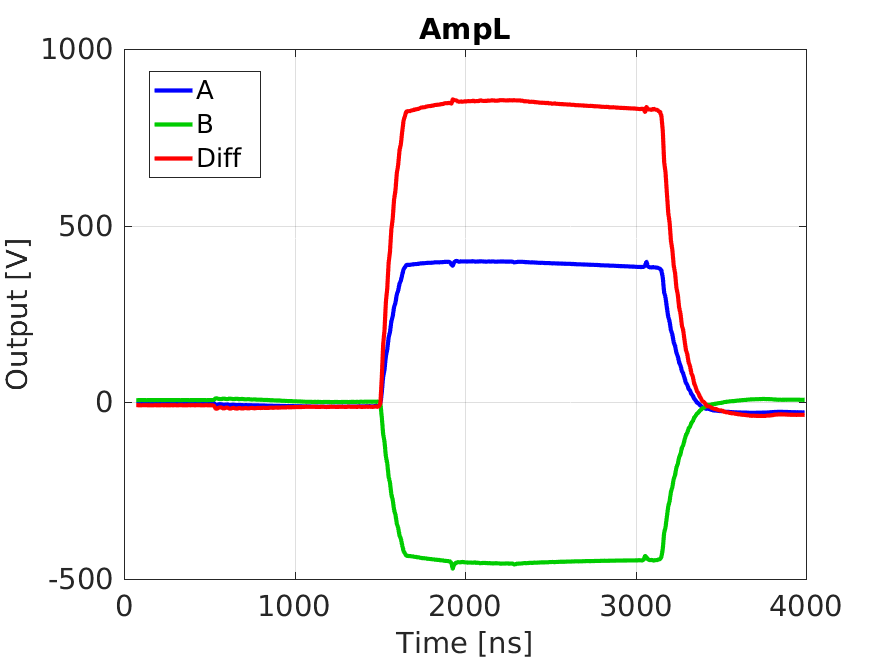
\includegraphics[width=0.8\textwidth]{Figures/commissioning/AmpL_Traces}
  \caption{The full output pulse of the A (blue) and B (green) channels for the left side of the amplifier, at an input voltage of \(+1\)~V. The difference between the A and B output is shown in red.}
  \label{f:ampLTraces}
  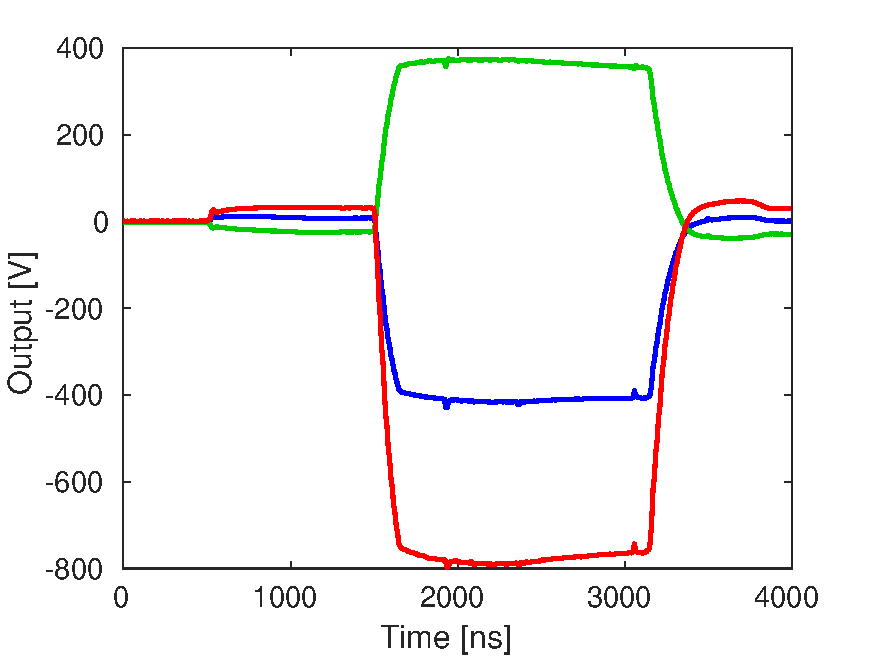
\includegraphics[width=0.8\textwidth]{Figures/commissioning/AmpR_Traces}
  \caption{The full output pulse of the A (blue) and B (green) channels for the right side of the amplifier, at an input voltage of \(-1\)~V. The difference between the A and B output is shown in red.}
  \label{f:ampRTraces}
\end{figure}

For each side of the amplifier both the A and B outputs are plotted as well as the difference of the two, which is the relevant quantity in terms of the kick received by the beam as it traverses the kickers. In the ideal case the potential difference should be flat along the full pulse length. However, for both the left and right side variations in the difference are visible, with an initial increase in output across the first 500~ns of the pulse followed by a droop in response across the second half of the pulse. Figure~\ref{f:ampFlatness} shows the peak-to-peak and mean deviation of the output voltage along the pulse across the full range of input voltages. The peak-to-peak deviation refers to the difference between the minimum and maximum output along the pulse, whilst the mean deviation is the average absolute difference between the mean output and the output at each sample point. For a constant input voltage the output voltage along the pulse varies by up to 88~V peak-to-peak (mean 12~V) for the left amplifier or 93~V peak-to-peak (mean 14~V) for the right amplifier. As a relative difference, this corresponds to approximately a 6~\% peak-to-peak, or 1~\% mean, variation along the pulse.

The PFF algorithm on the FONT5a board uses a single gain value across the whole pulse length for each correction output, thus making the approximation that the amplifier response is flat along the pulse. The variations along the amplifier pulse therefore directly translate in to discrepancies between the intended phase shift as calculated and the real phase shift experienced by the beam. As the region of interest for the correction is a few hundred nanoseconds about the central part of the pulse, as opposed to the full pulse length, the 1~\% mean variation is more indicative of the resulting error than the 6~\% peak-to-peak variation. With a correction range (Section \ref{ss:corrRange}) of \(\pm5.5^\circ\), the effects of the non-flat amplifier output should be below \(0.06^\circ\) and not measurable considering the phase monitor resolution of \(0.13^\circ\). Nevertheless, it could be foreseen to implement a droop correction in the PFF algorithm on the FONT5a board, taking the variations in the amplifier output along the pulse in to account.

\begin{figure}
  \centering
  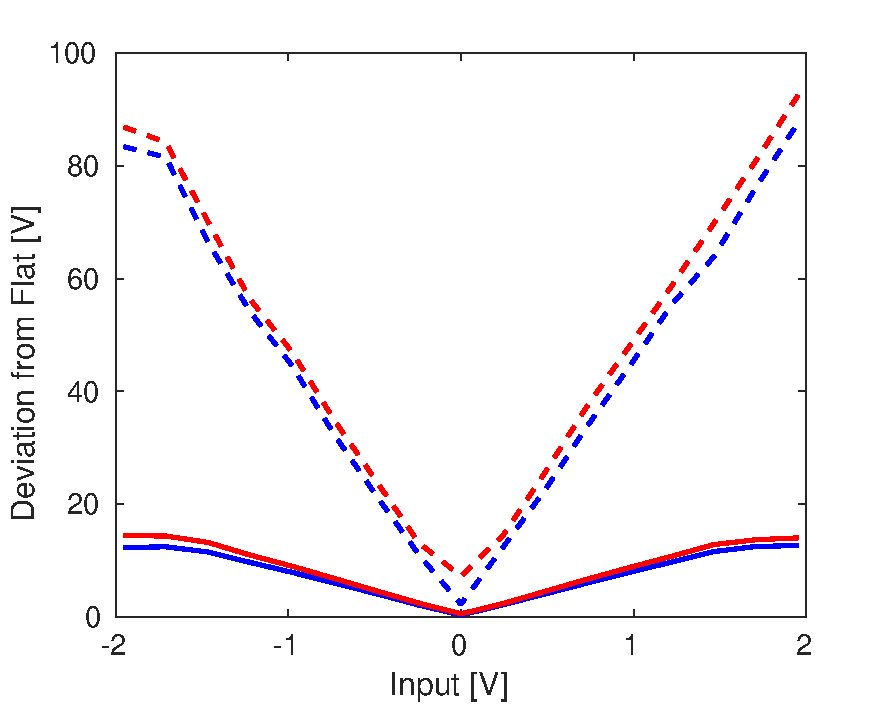
\includegraphics[width=0.8\textwidth]{Figures/commissioning/AmpFlatness}
  \caption{Peak-to-peak (dashed lines) and mean (solid lines) deviation from a flat output along the full amplifier output pulses for the left (blue) and right (red) side of the amplifier. The values are calculated using the difference between the A and B outputs of each side, the quantity relevant for kick experienced by the beam.}
  \label{f:ampFlatness}
\end{figure}

Variations in the amplifier output along the pulse can also lead to imperfect orbit closure in the chicane (as was discussed previously for differences in mean output). For this the relevant quantity is the sum of the potential difference sent to each kicker, or \((LA-LB)+(RA-RB)\). To ensure orbit closure this quantity, named the residual kick here, should be zero across the whole pulse length for all input voltages. Figure \ref{f:ampClosure} shows the residual kick along the pulse for all the input voltages in the scan. Clearly they are not all centred around zero, but this is expected due to the differences in the mean output voltage of the four amplifier outputs seen in Section~\ref{ss:ampLin}. As already stated, the overall mean offset could be removed by using a different gain for the two correction outputs. However, any variations along the pulse cannot be compensated for in the PFF algorithm. The magnitude of the effect is summarised in Figure \ref{f:ampClosureFlatness}, showing the peak-to-peak and average deviation of the residual kick from flat. The overall residual kick is very flat and the effect is smaller than any of those previously shown --- only up to 2~V on the mean or 21~V peak-to-peak.

\begin{figure}
  \centering
  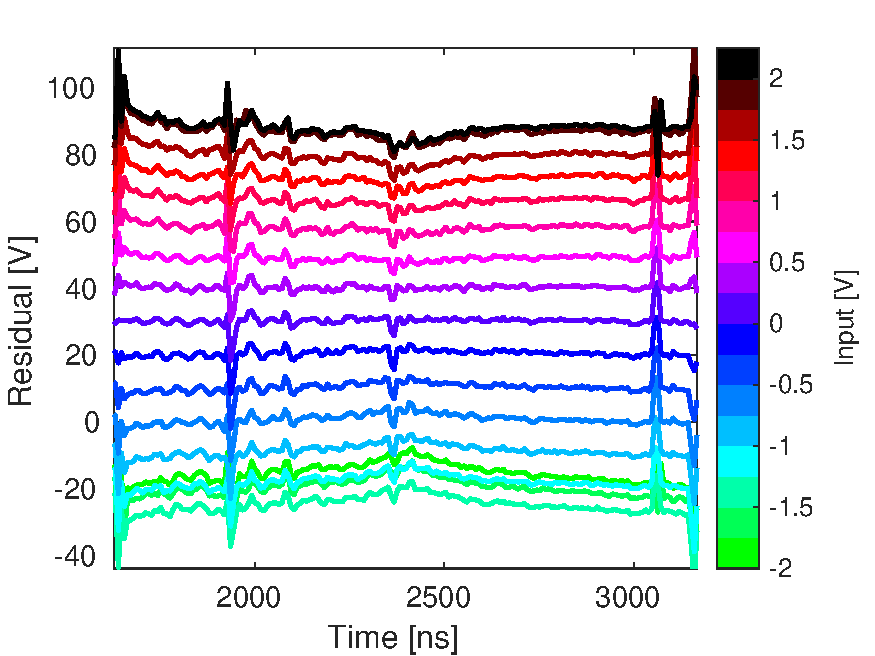
\includegraphics[width=0.8\textwidth]{Figures/commissioning/residualKick_Traces}
  \caption{Residual kick experienced by the beam after traversing the two kickers as a result of differences between the amplifier channels. The residual kick is the difference \((LA-LB)+(RA-RB)\) at each sample point. The residual is plotted for the full range of input voltages, as indicated by the colour scale.}
  \label{f:ampClosure}
  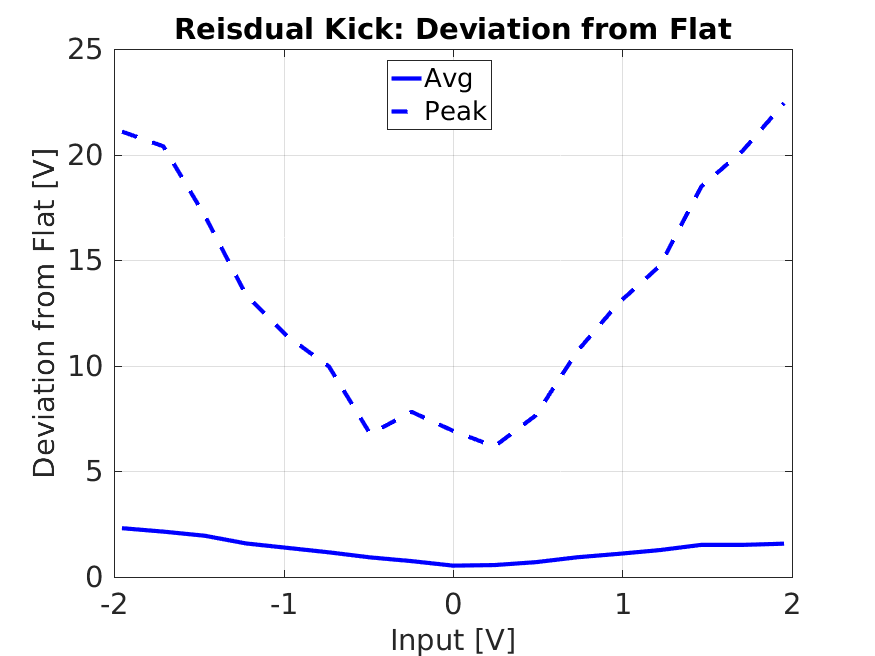
\includegraphics[width=0.8\textwidth]{Figures/commissioning/residualKick_Flatness}
  \caption{Peak-to-peak (dashed) and average (solid) deviation of the residual kick from Figure~\ref{f:ampClosure}. An ideal flat output pulse would give a deviation of zero.}
  \label{f:ampClosureFlatness}
\end{figure}

\newsection{daqSigProc}{Data Acquisition}

\subsection{Acquisition Tools}
\label{ss:acqTools}

\subsection{Monitoring Tools}
\label{ss:monTools}

Online display


\newsection{constKicks}{Kicker and Optics Performance Verification}

\subsection{Correction Range}
\label{ss:corrRange}

Knowledge of the correction range of the PFF system, or more specifically the relationship between the DAC output voltage from the FONT5a board and the resulting phase shift in the chicane, is critical for the PFF setup. In particular, it is needed to derive the optimal
correction gain, as seen in Section~\ref{ss:fontGain}.
%The first checks of the ability to shift the phase in the TL2 chicane using the new phase feedforward optics were performed with magnetic correctors prior to the PFF amplifier being available (these correctors can be used to implement a secondary ``Slow Correction'' to complement the PFF system, as discussed in Section~\ref{s:slowCorr}). 
%Aside from their use for the PFF correction, these tests and the clear variation with beam phase versus voltage sent to the PFF kickers shown in this section are already a significant achievement and a verification of the extensive work to improve the MADX model of TL2 presented in Chapter~\ref{c:tl2Optics}.


Figure \ref{f:phaseVsAmpVoltage} shows the mean phase shift after the chicane (in the downstream phase monitor) across the full \(\pm2\)~V input range of the amplifier. Constant DAC outputs in 17 steps between -4095 counts (-2~V) and +4095 counts (+2~V) were used to drive the amplifier. In order to reduce the sensitivity to any drifts in the beam phase between data points the scan was taken in interleaved mode, alternating between pulses with no drive to the amplifier and a constant non-zero DAC output. The phase plotted in Figure \ref{f:phaseVsAmpVoltage} is therefore the difference between 50 kicked beam pulses and 50 ``nominal'' pulses taken at the same time for each amplifier input voltage. 

\begin{figure}
  \centering
  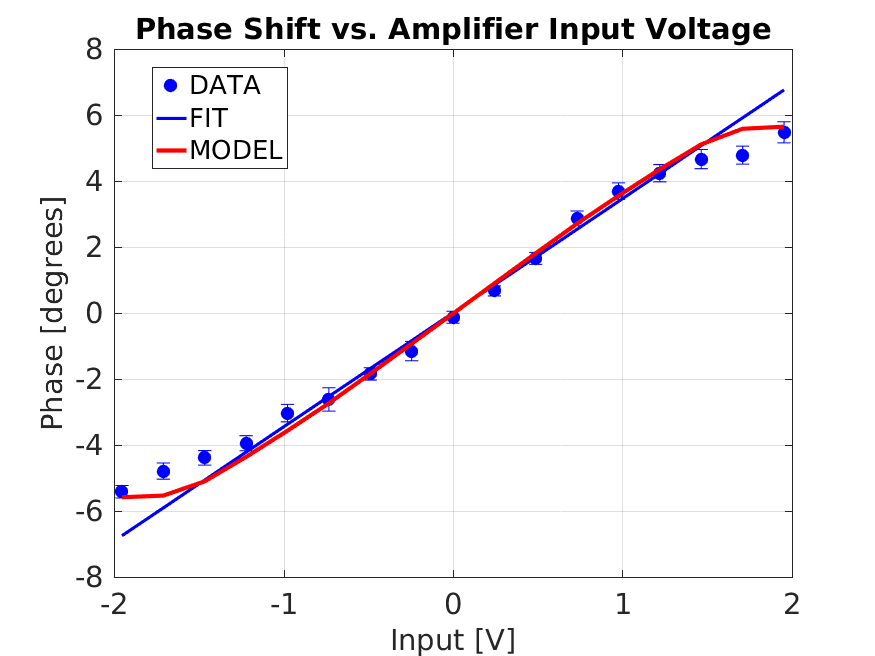
\includegraphics[width=0.8\textwidth]{Figures/commissioning/phaseVsAmpVoltage}
  \caption{Measured downstream phase shift versus amplifier input voltage (blue markers). The blue line shows a linear fit to the measured phase shift for inputs between \(\pm1.2\)~V. The red line shows the expected phase shift taking in to account the TL2 chicane optics, amplifier output voltage and kicker design (using Equation~\ref{e:ampVoltToPhase}.}
  \label{f:phaseVsAmpVoltage}
  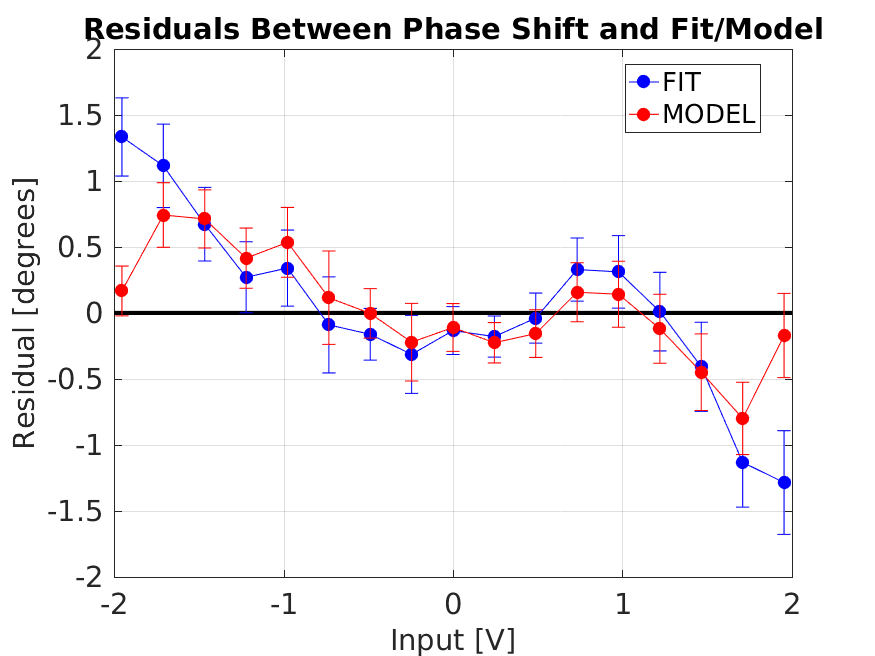
\includegraphics[width=0.8\textwidth]{Figures/commissioning/phaseVsAmpVoltage_residuals}
  \caption{Residuals between the measured phase shift and the expected (red) and fitted (blue) phase shifts from Figure~\ref{f:phaseVsAmpVoltage}.}
  \label{f:phaseVsAmp_resid}
\end{figure}

\begin{table}
  \begin{center}
    \begin{tabular}{| c | c | c |}
	   \hline
        & Phase Shift at +1~V Input & Max Phase Shift \\ \hline
       Data & \(3.5\pm0.1^\circ\) & \(5.5\pm0.3^\circ\) \\
	   Model & \(3.6^\circ\) & \(5.6^\circ\) \\
 	   \hline
    \end{tabular}
    \caption{Downstream phase shift resulting from an amplifier input of 1~V. The ``Data'' row shows the fitted gradient from the actual measured phase shift. The ``Model'' row shows the expected result given the known hardware and optics parameters.}
  	\label{t:PhaseVsDAC}
  \end{center}
\end{table}

At the maximum amplifier input voltage of \(2\)~V the phase after the chicane is shifted by \(5.5\pm0.3^\circ\). The fitted phase shift per Volt at the amplifier input is \(3.5\pm0.1^\circ\) in the \(\pm1.2\)~V linear input range of the amplifier. This fitted gradient is required and was previously introduced for the conversion between the PFF gain in the units on the FONT5a board and the real applied gain in Section~\ref{ss:pffFirmware}. In Section~\ref{ss:pffFirmware} it was quoted in terms of the phase shift in radians per DAC count output from the FONT5a board, rather than degrees per Volt as shown here. The value of \(30\mathrm{\mu rad/count}\) is easily derived using the conversion factors between degrees and radians and knowing that a DAC output of 4095 counts corresponds to 2~V sent to the amplifier.

Given knowledge of the amplifier output characteristics (Section~\ref{ss:ampLin}), the kicker specifications (Section~\ref{s:kickers}) and the chicane optics (Section~\ref{s:matchedOptics}) the real phase shift seen in the scan can be compared to the expected phase shift based on the system parameters. The predicted phase shift, \(\Delta\phi\), in degrees is given by:
\begin{equation}
 	\Delta\phi = V_{amp}[V_{font}].K.R_{52}.\frac{360}{\lambda_{12\mathrm{GHz}}}
 	\label{e:ampVoltToPhase}
\end{equation} 
Where \(V_{amp}[V_{font}]\) is the amplifier output Voltage at an input voltage of \(V_{font}\) sent from the FONT5a board, \(K\) is the angular deflection of the beam per Volt applied to each kicker strip, \(R_{52}\) is the \(R_{52}\) value between the kickers in the PFF optics and \(\frac{360}{\lambda_{12\mathrm{GHz}}}\) converts the calculated orbit length difference in to an equivalent 12~GHz phase using the 12~GHz wavelength \(\lambda_{12\mathrm{GHz}}\). The value of most of these parameters has already been derived in the sections previously mentioned. They are:
\begin{eqnarray*}
V_{amp}[1~\mathrm{V}] = 435~\mathrm{V} \\
K = 0.8~\mathrm{\mu rad/V}\\
R_{52} = -0.7~\mathrm{m}\\
\lambda_{12\mathrm{GHz}} = 2.5~\mathrm{cm} 
\end{eqnarray*}
The value of \(V_{amp}[1~\mathrm{V}]\) is given as a representative value in the linear range of the amplifier but the actual amplifier output at all input voltages is used in the predictions to include the effects of saturation in the calculated phase shift values. Also, the output from the left side of the amplifier, applied to the first kicker, is used as this is most relevant for the phase shift in the chicane (the orbit should be closed after the second kicker with no further phase shift in the chicane after that point). The value of \(K\) is derived from the kicker design, in which 1.4~kV applied to each strip gives a 1~mrad kick for a 150~MeV beam \cite{kickerIPAC11}.  The actual CTF3 beam energy is approximately 135~MeV (calculated based on the dipole currents used in the machine setup), so the value of \(K\) above is scaled by a factor 150/135.

In Figure~\ref{f:phaseVsAmpVoltage} the predicted phase shifts using Equation~\ref{e:ampVoltToPhase} are also shown. Table~\ref{t:PhaseVsDAC} compares the fitted gradients and maximum phase shift for the model and the measurement. The overall agreement between the two is good, with the residuals between the model and the data generally consistent with zero within error bars in the \(\pm1.2\)~V linear range of the amplifier as shown in Figure~\ref{f:phaseVsAmp_resid}. The residuals between the data and the linear 
fit to the data are also consistent with zero in this range.

Outside the linear range some discrepancies appear, with the difference being largest where the amplifier has started to enter saturation but before it has reached peak output. 
%However, most amplifier effects can be excluded as the analysis in this section uses the same dataset that was used to characterise the amplifier performance in Section~\ref{s:amplifierSetup}. 
The actual amplifier output voltage at all inputs (from
 Section~\ref{s:amplifierSetup}) is used to calculate the expected phase shift shown in the figure. This means any differences between the measured and expected results are unlikely to be related to the amplifier.
Possible explanations could be remaining higher order errors in the TL2 chicane optics, or unexpected behaviour from the kickers or amplifier. Although subtracting alternating, interleaved pulses should remove the sensitivity to drifts in the machine it is possible that some residual effect remains. To determine whether the discrepancies are reproducible further scans of this type will need to be completed in the future. The residuals between between the data and the linear fit between \(\pm1.2\)~V would also be of significance for the PFF correction should they not converge to zero with additional measurements, as they are of similar magnitude to the \(0.2^\circ\) downstream jitter target. 

However, the overall conclusion is as expected --- the phase shift in the chicane linearly depends on the amplifier input in the \(\pm1.2\)~V (\(\pm2500\) DAC counts) region thus a close to optimal correction can be applied in this range, corresponding to a \(\pm4.2\pm0.1^\circ\) phase shift. When the calculated optimal correction is between an absolute input voltage of 1.2~V and 2.0~V, 2500 to 4096 DAC counts, or \(\pm4.2\pm0.1^\circ\) to \(\pm7.0\pm0.2^\circ\), the actual phase shift in the chicane is lower, only up to \(\pm5.5\pm0.3^\circ\), due to the amplifier entering saturation (and possibly other effects to be determined ). Any calculated correction outside \(\pm5.5\pm0.3^\circ\) receives a static phase shift of \(\pm5.5\pm0.3^\circ\) in the chicane. In the limit where all pulses are outside this range the PFF system can only induce a static shift in the mean phase and makes no improvement to the phase jitter. The effect of limited correction range on the most recent PFF results is seen in Section~\ref{s:longFF_singleResults}.

Aside from its use for the PFF setup demonstrating the ability
 to shift the phase in the TL2 chicane is already a significant 
 achievement. In particular a phase shift is only possible if 
 \(R_{52}\) is non-zero between the kickers in the optics for the
 chicane (Section~\ref{ss:pffOpticsReqs}). The agreement between the
 modelled and measured correction range verifies the optics is 
 performing as expected, which would not have been possible without
 the improvements made to the MADX model of the line in
 Section~\ref{s:opticsMeas}. It also shows the kickers are performing
 as per their design, imparting the expected angular deflection to
 the beam for the applied voltage from the amplifier.

%\subsection{Variations Along Pulse}
%\label{ss:kickPulseVar}
%
%[TODO: In this section I intended to check the stability of the constant kick along the pulse, as I did for the "Shape" section with the amplifier above. The results from the constant kick data do not look good, though - the errors are quite large and there are some nasty oscillations along the pulse, such as in the example Figure~\ref{f:phaseShiftAlongConstKick}. With the phase stability downstream a much longer scan would probably be needed to draw conclusions here, though even on longer time scales I think it needs to be checked that the difference between odd and even pulses converges to zero. As it is I would probably choose to skip this section, or possibly just show one of the better plots.]
%
%\begin{figure}
%  \centering
%  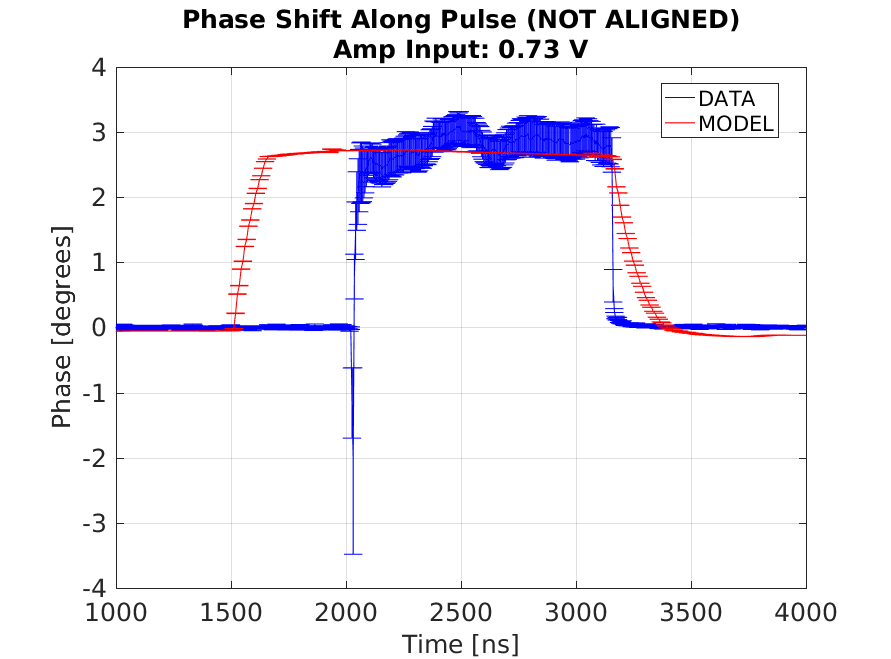
\includegraphics[width=0.8\textwidth]{Figures/commissioning/phaseShiftAlong}
%  \caption{Traces relative timing scan.}
%  \label{f:phaseShiftAlongConstKick}
%\end{figure}

\subsection{Correction Shape}
\label{ss:kickShape}

The previous result in Section~\ref{ss:corrRange} demonstrates that the kickers in the chicane can be used to shift the mean beam phase. However, the PFF correction also aims to remove variations in the phase point by point along the beam pulse. In the PFF algorithm the DAC output is varied along the pulse based on the measured upstream phase in order to achieve this, rather than being constant as has been the case in the tests presented up until this point. The amplifier and kickers must then have sufficient bandwidth to respond to fast changes in input voltage, in order to ultimately remove these features from the corrected downstream phase.

\begin{figure}
  \centering
  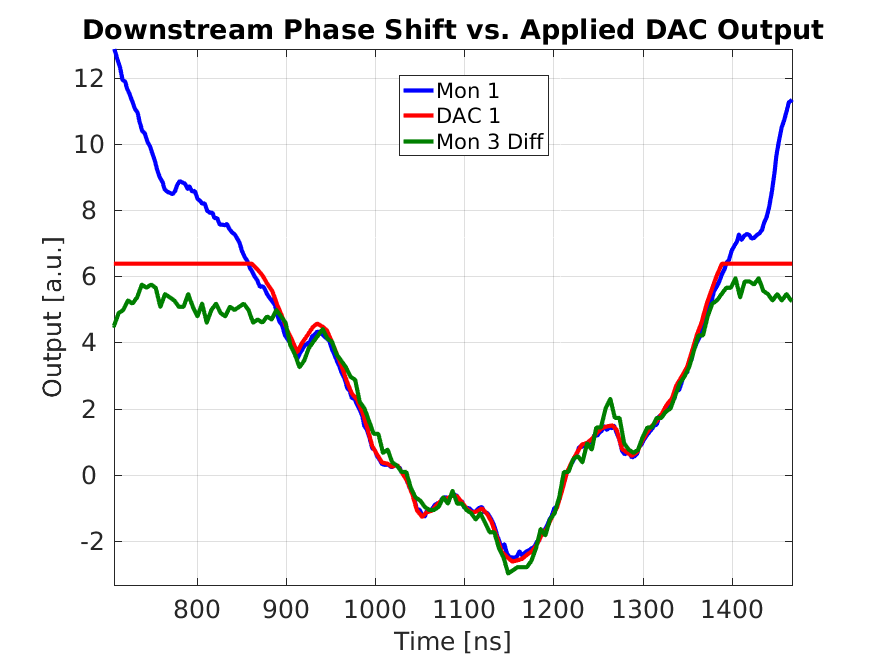
\includegraphics[width=0.8\textwidth]{Figures/commissioning/pffKickShape}
  \caption{Comparison between the upstream phase (blue), used as the PFF input, the resulting DAC output from the FONT5a board (red) and the measured downstream phase shift as a result of the applied kick (green).}
  \label{f:pffKickShape}
\end{figure}

To verify that the FONT5a board, amplifiers and kickers respond as expected Figure~\ref{f:pffKickShape} shows the first example in the thesis of results with the complete PFF system turned on. 
The input upstream phase, calculated DAC output and the observed difference in the downstream phase resulting from the applied kick are all shown. The downstream phase trace shows the difference between subsequent pulses with the correction on and off (using the interleaved correction mode). 

In the ideal case the shape of all three lines should be identical, apart from the DAC output and downstream phase shift having opposite sign to the input upstream phase (in order to remove the upstream phase variations from the corrected downstream phase).
Each trace is scaled, aligned in time and sign flipped where appropriate to make a comparison between the shapes easier.
When operating the PFF system to reduce the downstream jitter as intended these scale factors and times must be applied in the PFF
setup rather than in offline data analysis. The scale factor is analogous to the system gain, for which the optimal value is derived
in Section~\ref{ss:fontGain}, and the correction output timing is
discussed in Section~\ref{s:timing}.

In the central region of the pulse all three traces have the same shape as expected. The upstream phase and DAC output should be close to identical by definition, as the calculated correction output is only dependent on the input phase, but this verifies the functionality of the FONT5a board correction algorithm and firmware. The agreement in shape of the downstream phase shift is a significant achievement, and verifies the linearity of the amplifier output, kicker response and optics for a varying input voltage. This result demonstrates that everything is in place for the PFF prototype to flatten variations in the downstream phase and to reduce the downstream phase jitter.

The agreement in shape holds for times between around 900~ns and 1375~ns as indicated on the figure, and this defines a 475~ns portion of the pulse within which the applied correction should be close to optimal. Outside this range the large phase sag along the pulse leads 
to the correction being saturated -- the maximum possible DAC output 
(2~V) is applied and the shape can no longer be corrected. It can also
be seen that the measured downstream phase shift saturates earlier than
the applied DAC output. This is because the amplifier begins to 
saturate at input voltages below 2~V, as seen in Figure~\ref{f:AmpOutvsDAC}.

\subsection{Orbit Closure}
\label{ss:orbitClosure}

At CLIC the PFF system must not degrade the transverse beam stability. This means for any voltage sent to the kickers the horizontal beam orbit after the PFF chicane must be unchanged, or closed, despite the different orbits inside the chicane. As such, the PFF optics for the TL2 chicane at CTF3 is also designed to give a closed kick, as presented in Section~\ref{s:matchedOptics}. However, up until now the main focus during PFF operation has been the primary goal of reducing the downstream phase jitter and ensuring good beam transmission to the downstream phase monitor. As a result orbit closure after the TL2 chicane has not yet been strictly enforced during PFF operation as will be seen in this section, but the current status is shown here as an additional cross-check of the PFF optics and to highlight where improvements are needed for future tests.

Using the same constant kick data as Section~\ref{ss:corrRange}, Figure~\ref{f:HOrbitVsInput} shows mean the horizontal orbit before, inside and after the TL2 chicane across the full \(\pm2\)~V range of amplifier input voltages. Two BPMs before and after the chicane, as well as the four inside the chicane, are included. The plotted positions are the difference between the kicked and nominal (non-kicked) orbit at each BPM, thus removing any misalignment in the BPM centres. Before the chicane and the first kicker there is no significant effect on the orbit as expected. Inside the chicane the PFF system induces an orbit offset of up to \(1.4\pm0.1\)~mm. After the chicane, in BPMs CC.845 and CC.930, the orbit should return to zero in the ideal case. However, a clear residual offset can be seen, up to \(0.5\pm0.1\)~mm in CC.930.

\begin{figure}
  \centering
  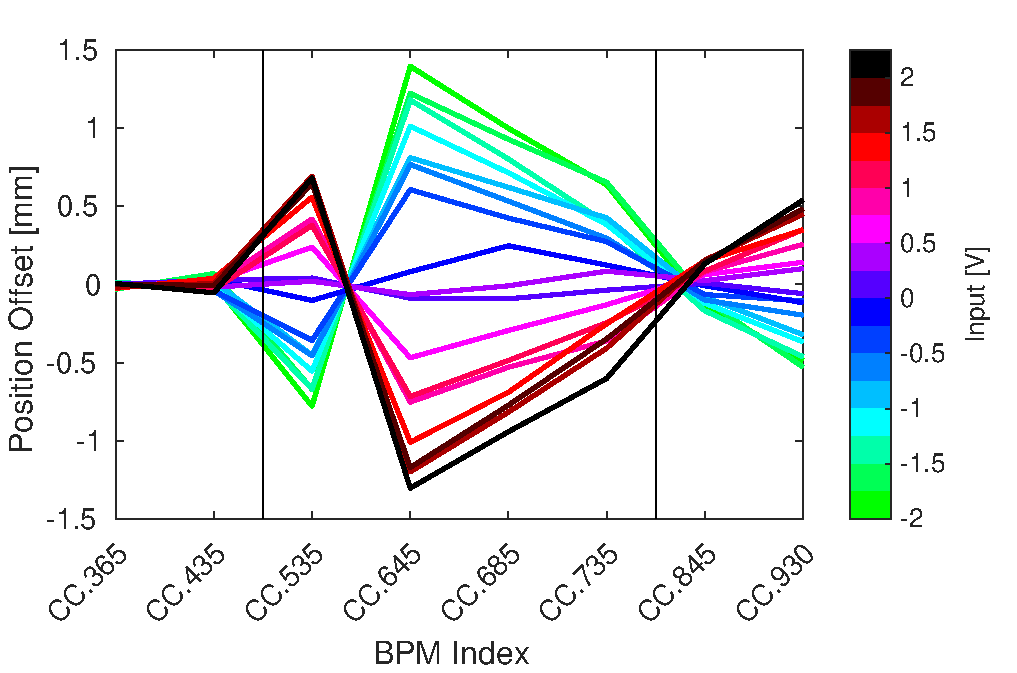
\includegraphics[width=0.85\textwidth]{Figures/commissioning/HOrbitVsInput}
  \caption{Horizontal orbit offset in and around the TL2 chicane at different amplifier input voltages (as indicated by the colour scale). The approximate positions of the chicane entrance and exit are indicated by vertical black lines. The two PFF kickers are located at index CC.480 and CC.780 (before the first and last dipoles in the chicane).}
  \label{f:HOrbitVsInput}
    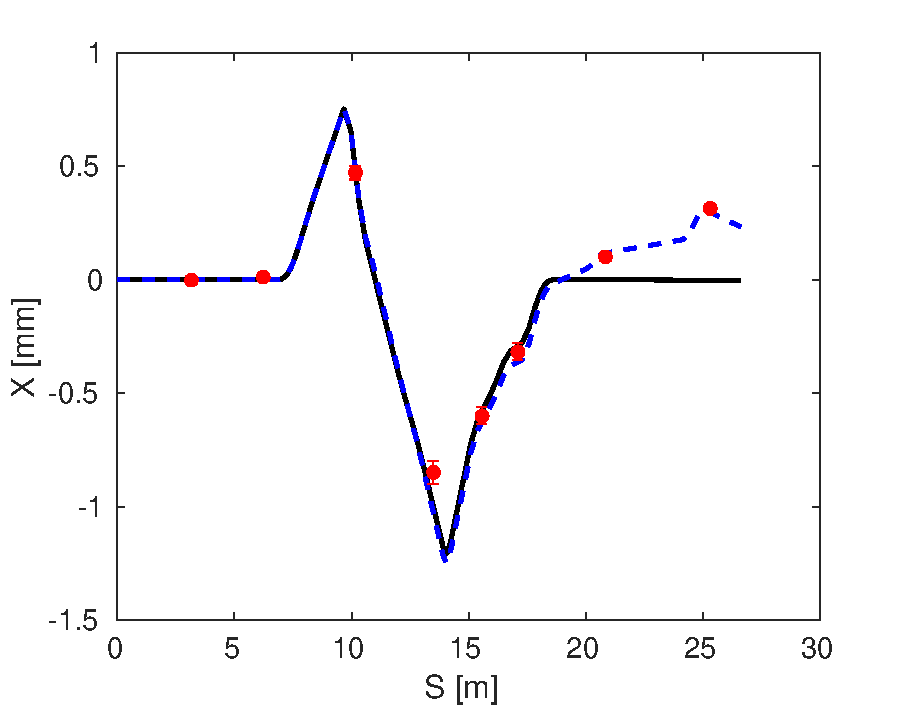
\includegraphics[width=0.75\textwidth]{Figures/commissioning/orbClosureVsQuadModel}
  \caption{Orbit in the TL2 chicane at 1~V amplifier input for the BPM data (red markers), nominal model (black line) and the model taking in to account the actual quadrupole currents used in TL2 at this time (dashed blue line). Vertical black lines mark the entrance and exit
   of the chicane.}
  \label{f:orbClosureVsQuadModel}
\end{figure}

%\begin{figure}
%  \centering
%%  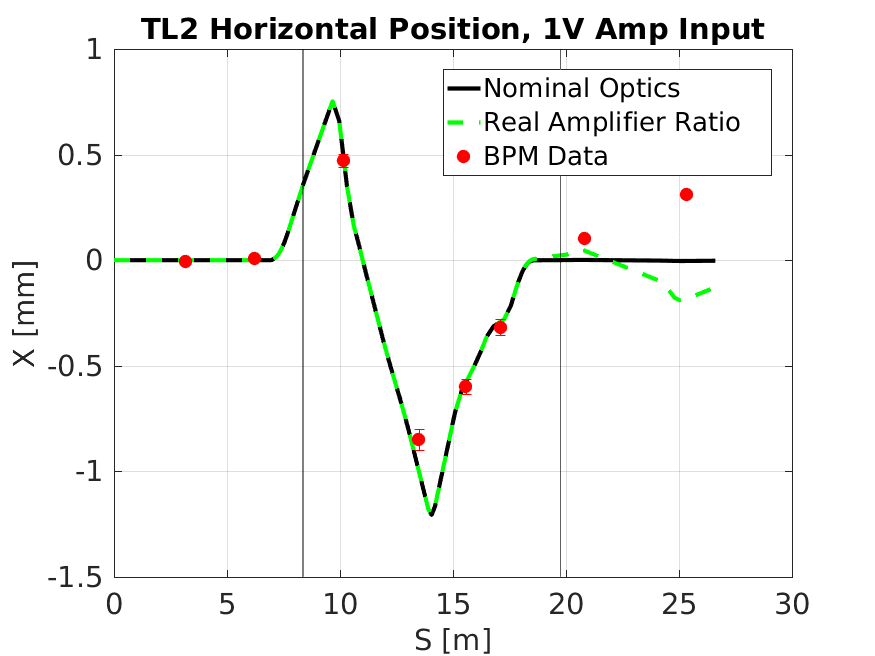
\includegraphics[width=0.8\textwidth]{Figures/commissioning/orbClosureVsAmpModel}
%%  \caption{Orbit in the TL2 chicane at 1~V amplifier input for the BPM data (red markers), nominal model (black line) and the model taking in to account the small differences between each amplifier output (dashed green line).}
%%  \label{f:orbClosureVsAmpModel}
%  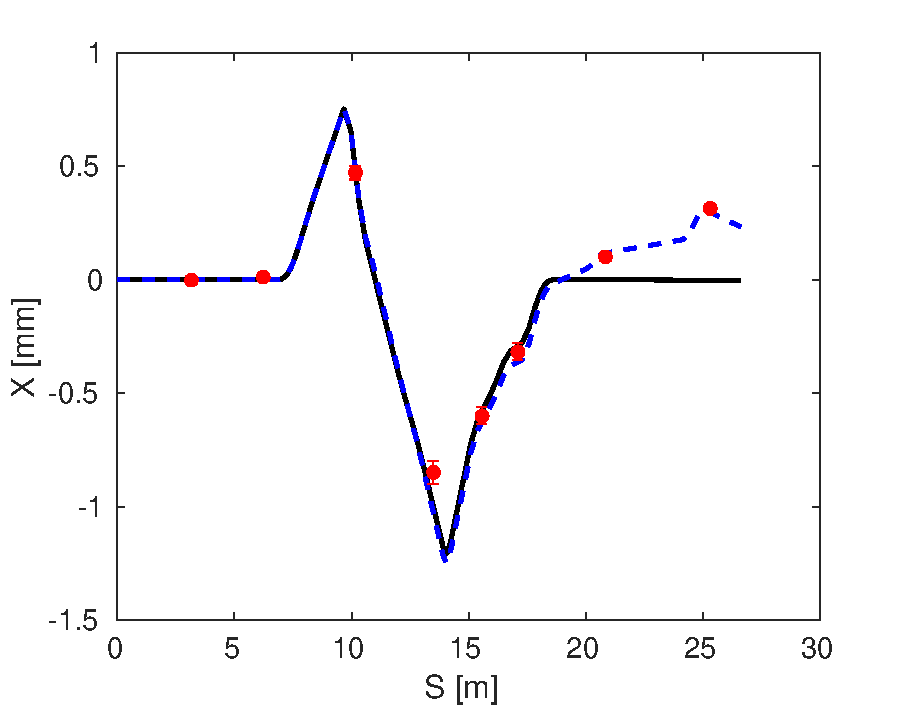
\includegraphics[width=0.75\textwidth]{Figures/commissioning/orbClosureVsQuadModel}
%  \caption{Orbit in the TL2 chicane at 1~V amplifier input for the BPM data (red markers), nominal model (black line) and the model taking in to account the actual quadrupole currents used in TL2 at this time (dashed blue line). Vertical black lines mark the entrance and exit
%   of the chicane.}
%  \label{f:orbClosureVsQuadModel}
%\end{figure}

%The true explanation for the non-closed orbit is that the quadrupole strengths used in the machine setup are not exactly nominal. 
Although every effort has been made to keep the TL2 optics as close to nominal as possible, particularly inside the chicane, it is an extremely sensitive area for the setup of CTF3 and beam transport in to the CLEX area downstream of TL2 (including the location of the downstream phase monitor in the TBL line) is always difficult \cite{piotrPriv}. Minor modifications have therefore been necessary in order to achieve full beam transmission to the downstream area, both for PFF and other experiments at CTF3. The largest changes have been made to the four quadrupoles following the chicane but one quadrupole inside the chicane, CC.IQFL0730 (just prior to the 2nd kicker) has a set value \(10\%\) lower than the nominal optics, as well as differences up to \(2\%\) in the other quadrupoles. 

Figure~\ref{f:orbClosureVsQuadModel} compares the measured beam orbit
 in the BPMs to the expected response in the PFF optics with the 
 nominal quadrupole strengths, and the expected response taking in to
 account the actual quadrupole strengths used in this dataset.
 The full MADX orbit propagated through all elements is shown, with the eight measured BPM offsets included at their respective positions. 
 Each BPM point represents the gradient of a linear fit using the variation with input voltage seen previously in Figure~\ref{f:HOrbitVsInput}.
 Before and inside the chicane the agreement between the BPM data and both models is excellent.
  After the chicane the orbit is closed in the nominal optics but the 
  measured position offset in the BPMs is non-zero, as seen previously.
  However, there is excellent agreement between the measured positions
  and the expected response in the MADX model taking in to account the 
  actual quadrupole strengths applied in TL2 during this dataset.

This gives confidence that if a completely nominal optics could be 
used in TL2 orbit closure would be obtained. For future tests attempts 
will be made to further optimise the setup of CTF3 and allow a 
completely nominal optics to be used in TL2. It should also be 
noted that for these tests both sides of the amplifier were driven with the same magnitude input voltage. This has also been the case for 
all the PFF correction attempts presented in Chapter~\ref{c:feedforward}. 
However, in Section~\ref{ss:ampLin} it was seen that the right side of the amplifier (powering the second kicker) gave 4\% lower output than the left side (powering the first kicker).
To strictly enforce orbit closure with a nominal optics it would 
therefore be necessary to drive the right side of the amplifier with 
a 4\% higher input voltage (by using a 4\% higher gain for the DAC2 
output compared to the DAC1 output on the FONT5a board).



%Using the actual quadrupole strengths used in the machine gives the result shown in Figure \ref{f:orbClosureVsQuadModel}. In this case the agreement between the model and the data is also extremely good after the chicane. It may still be possible to compensate for these differences by outputting different voltages to each kicker and this will be investigated. Alternatively, a completely nominal optics can be set in the chicane purely for the purposes of verifying orbit closure, reverting back to non-nominal optics and closure if needed to achieve good beam transmission for normal PFF operation.

%During this scan both sides of the amplifier were driven with the same magnitude input voltage. However, in Section~\ref{ss:ampLin} it was seen that the right side of the amplifier (powering the second kicker), gave 4\% lower output than the left side. This could explain why the orbit after the chicane was not closed during this scan, and during PFF operation which has typically used equal gain for both correction outputs to date. Figure~\ref{f:orbClosureVsAmpModel} shows the expected orbit in the TL2 chicane in the case where both kickers are driven with the same voltage (``nominal optics'') and with the 2nd driven with a 4\% lower voltage (``real amplifier ratio'').
%\footnote{The term ``nominal optics" is used in this section to refer to the nominal PFF optics, not the nominal optics created in Chapter~\ref{c:tl2Optics} to use when the PFF system is not under operation.}
%The full MADX orbit propagated through all elements is shown, with the eight real measured BPM offsets also included at their respective positions. Each BPM point represents the gradient of a linear fit using the variation with input voltage seen previously in Figure~\ref{f:HOrbitVsInput}. Before and inside the chicane the agreement between the BPM data and the model is excellent. As seen before, the BPM orbit is not closed after the chicane, unlike the nominal optics. If the actual kicker voltage ratio is taken in to account the MADX orbit after the chicane is not closed either, but the offset has opposite polarity to the real data in the last BPM.



\newsection{timing}{Correction Output Timing}

Most the results based on the amplifier outputs and kicked beam presented so far have used a constant output voltage sent from the FONT5a board across the full \(1.4~\mathrm{\mu s}\) time window that the amplifier is powered for. As the \(1.4~\mathrm{\mu s}\) amplifier output sent to the kickers is much longer than the \(1.1~\mathrm{\mu s}\) CTF3 beam pulse it is relatively straightforward to ensure that the full length of the pulse experiences the constant kick with this setup. However, for operation of the PFF system precise control of the correction output timing becomes critical. In order to remove phase variations along the pulse with the PFF system the output correction signal, shaped by the upstream phase, must arrive at the kickers exactly in sync with the beam. Any timing misalignment between the beam and correction signal arrival will result in residual oscillations along the pulse in the downstream phase, even in the case where the upstream-downstream phase propagation is perfect. Approximating the phase sag along the pulse to be quadratic, \(\phi_{u}(t) \sim \phi_{d}(t) \sim t^2\), a misaligned correction would yield a corrected downstream phase with a linear increase in phase along the pulse with time, \(\phi_{PFF}(t)~\sim~\phi_d(t)-\phi_u(t+\delta)~\sim -2\delta t - \delta^2\), for example, where \(\phi_{PFF}\) is the corrected phase, \(\phi_{d}\) the uncorrected downstream phase, \(\phi_{u}\) the upstream phase, \(t\) the time and \(\delta\) the time misalignment in the applied correction. Also, the effect is particularly significant for any higher frequency variations in phase along the pulse. If a 40~ns oscillation is present in the upstream phase but the correction is applied with a 50~ns delay, for example, a second 40~ns oscillation with opposite sign would be introduced to the ``corrected'' downstream phase at a later time with no change to the initial oscillation. Although the effects are most visible along the pulse, any timing delay will also degrade the achievable mean phase jitter. This section gives an overview of the main methods that have been used to ensure that the correction output to the two kickers arrives in time with the beam. 

\subsection{Kicker Cable Lengths}
\label{ss:kickerCables}

The cables carrying the correction signal between the PFF amplifier and the kickers in the TL2 chicane are the single largest contributor to the overall system latency. They must be routed from the PFF electronics racks (in the klystron gallery, one floor and directly above the location of the upstream phase monitors), down in to the machine hall and across the width of the CTF3 facility to the TL2 chicane. The initial kicker cables installation used pre-existing cable trays and gave a signal transit time of 260~ns, with a signal speed of 0.66~c and approximate lengths of 50~m. This is more than two thirds the overall PFF latency budget, which must be lower than the 380~ns beam time of flight between the upstream phase monitor and the first kicker. Considering the latencies of the various pieces of hardware in the PFF system chain as well as the cables between the upstream phase monitors and the PFF electronics (Section~\ref{ss:availLatency}), the overall PFF system latency would have been in excess of the \(380\)~ns beam time of flight with this setup. By re-routing the cables on to a dedicated pathway and trimming any remaining slack it was possible to reduce the cable lengths by up to 90~ns, bringing the system within the latency budget as will be seen in the following sections. Precise measurements of the cable lengths with this setup are presented in this section, as well as their significance beyond ensuring the system is within the latency requirements.

With two kickers, two strips per kicker and two ends of each strip a total of eight cables are needed. The drive from the amplifier is applied to the downstream end of each kicker strip, traverses the kicker, and is then terminated back at the amplifier after leaving the upstream end. Drive is applied to the downstream end of each kicker (meaning it propagates through the kicker in the opposite direction to the beam) so that the electric and magnetic fields between the strips are in the same direction, as discussed in Section~\ref{s:kickers}. Rather than being connected directly to the amplifier, the eight kicker cables are connected to a patch panel below the amplifier in the PFF electronics racks. Eight additional cables, around 70~cm in length, are used to connect the amplifier outputs to the patch panel. This is in order to create a tidier cabling setup in the rack as well as making changes to the amplifier cabling easier, when necessary. The patch panel also deals with the conversion between HN-type connectors (used on the kickers and kicker cables) and N-type connectors (used on the patch panel cables and to connect to the amplifier after a further transition to TNC connectors \ref{colinCLIC16}).

The length of the eight kicker cables and eight patch panel cables has been measured using time domain reflectometry (TDR) on a network analyser. The network analyser is used to send a short pulse down the cable,  with one end of the cable connected to the network analyser and the other end disconnected so it is not correctly terminated. As the signal reaches the (non-terminated) end of the cable the discontinuity in impedance creates a reflected signal that propagates back to the network analyser. The time difference between when the signal was output and when the reflected signal arrives back at the network analyser therefore corresponds to double the one-way signal transit time in the cable.

Table~\ref{t:shortCabLengths} shows the patch panel cable lengths and Table~\ref{t:kickCabLengths} the kicker cable lengths that were determined with this method. Quoted errors of \(\pm0.05\)~ns are estimated based on the sampling rate of the measurement. The amplifier port, patch panel port and kicker strip that the cables are connected to are also shown in the table, as well as their corresponding CTF3 identifying number for reference. For the amplifier port labels the three letters correspond to:
\begin{itemize}
\item Whether the cable is connected to the \textbf{L}eft or \textbf{R}ight side of the amplifier.
\item  Whether the cable is connected to the amplifier \textbf{A} or \textbf{B} outputs on that side.
\item Whether the cable is connected to the amplifier \textbf{D}rive or \textbf{T}erminator.
\end{itemize}
And for the kicker strip labels the three letters correspond to:
\begin{itemize}
\item Whether the cable is connected to the first (\textbf{1}) or second (\textbf{2}) kicker.
\item  Whether the cable is connected to the \textbf{U}pstream or \textbf{D}ownstream end of the kicker strip.
\item Whether the cable is connected to the \textbf{L}eft or \textbf{R}ight kicker strip, as viewed looking at the upstream end of the kicker.
\end{itemize}
Finally, the patch panel connectors are simply labelled from 1 to 8 from left to right, as viewed from the front of the rack. All of the cable connections between the amplifier, patch panel and kickers are shown in Figure~\ref{f:kickerCables}.

\begin{table}
  \begin{center}
    \begin{tabular}{| c | c | c | c | c |}
	   \hline
       Label & Length & Amplifier Port & Patch Panel Port \\ \hline
       2907701B & \(2.99\pm0.05\)~ns & LAT & 1 \\
       2907703B & \(3.03\pm0.05\)~ns & LBT & 2 \\
       2907700B & \(3.03\pm0.05\)~ns & LAD & 3 \\
       2907702B & \(3.01\pm0.05\)~ns & LBD & 4 \\
       2907838B & \(3.03\pm0.05\)~ns & RAD & 5 \\
       2907740B & \(3.05\pm0.05\)~ns & RBD & 6 \\
       2907739B & \(3.03\pm0.05\)~ns & RAT & 7 \\
       2907741B & \(3.03\pm0.05\)~ns & RBT & 8 \\
 	   \hline
    \end{tabular}
    \caption{Lengths of cables between the amplifier and the patch panel.}
  	\label{t:shortCabLengths}
  \end{center}
\end{table}

\begin{table}
  \begin{center}
    \begin{tabular}{| c | c | c | c | c |}
	   \hline
       Label & Length & Patch Panel Port & Kicker Strip \\ \hline
       2907701A & \(171.28\pm0.05\)~ns & 1 & 1UL \\
       2907703A & \(171.30\pm0.05\)~ns & 2 & 1UR \\
       2907700A & \(171.29\pm0.05\)~ns & 3 & 1DL \\
       2907702A & \(171.30\pm0.05\)~ns & 4 & 1DR \\
       2907838A & \(205.45\pm0.05\)~ns & 5 & 2DL \\
       2907740A & \(205.62\pm0.05\)~ns & 6 & 2DR \\
       2907739A & \(205.15\pm0.05\)~ns & 7 & 2UL \\
       2907741A & \(204.49\pm0.05\)~ns & 8 & 2UR \\
 	   \hline
    \end{tabular}
    \caption{Lengths of cables between the patch panel and the kickers.}
  	\label{t:kickCabLengths}
  \end{center}
\end{table}


\begin{figure}
  \centering
  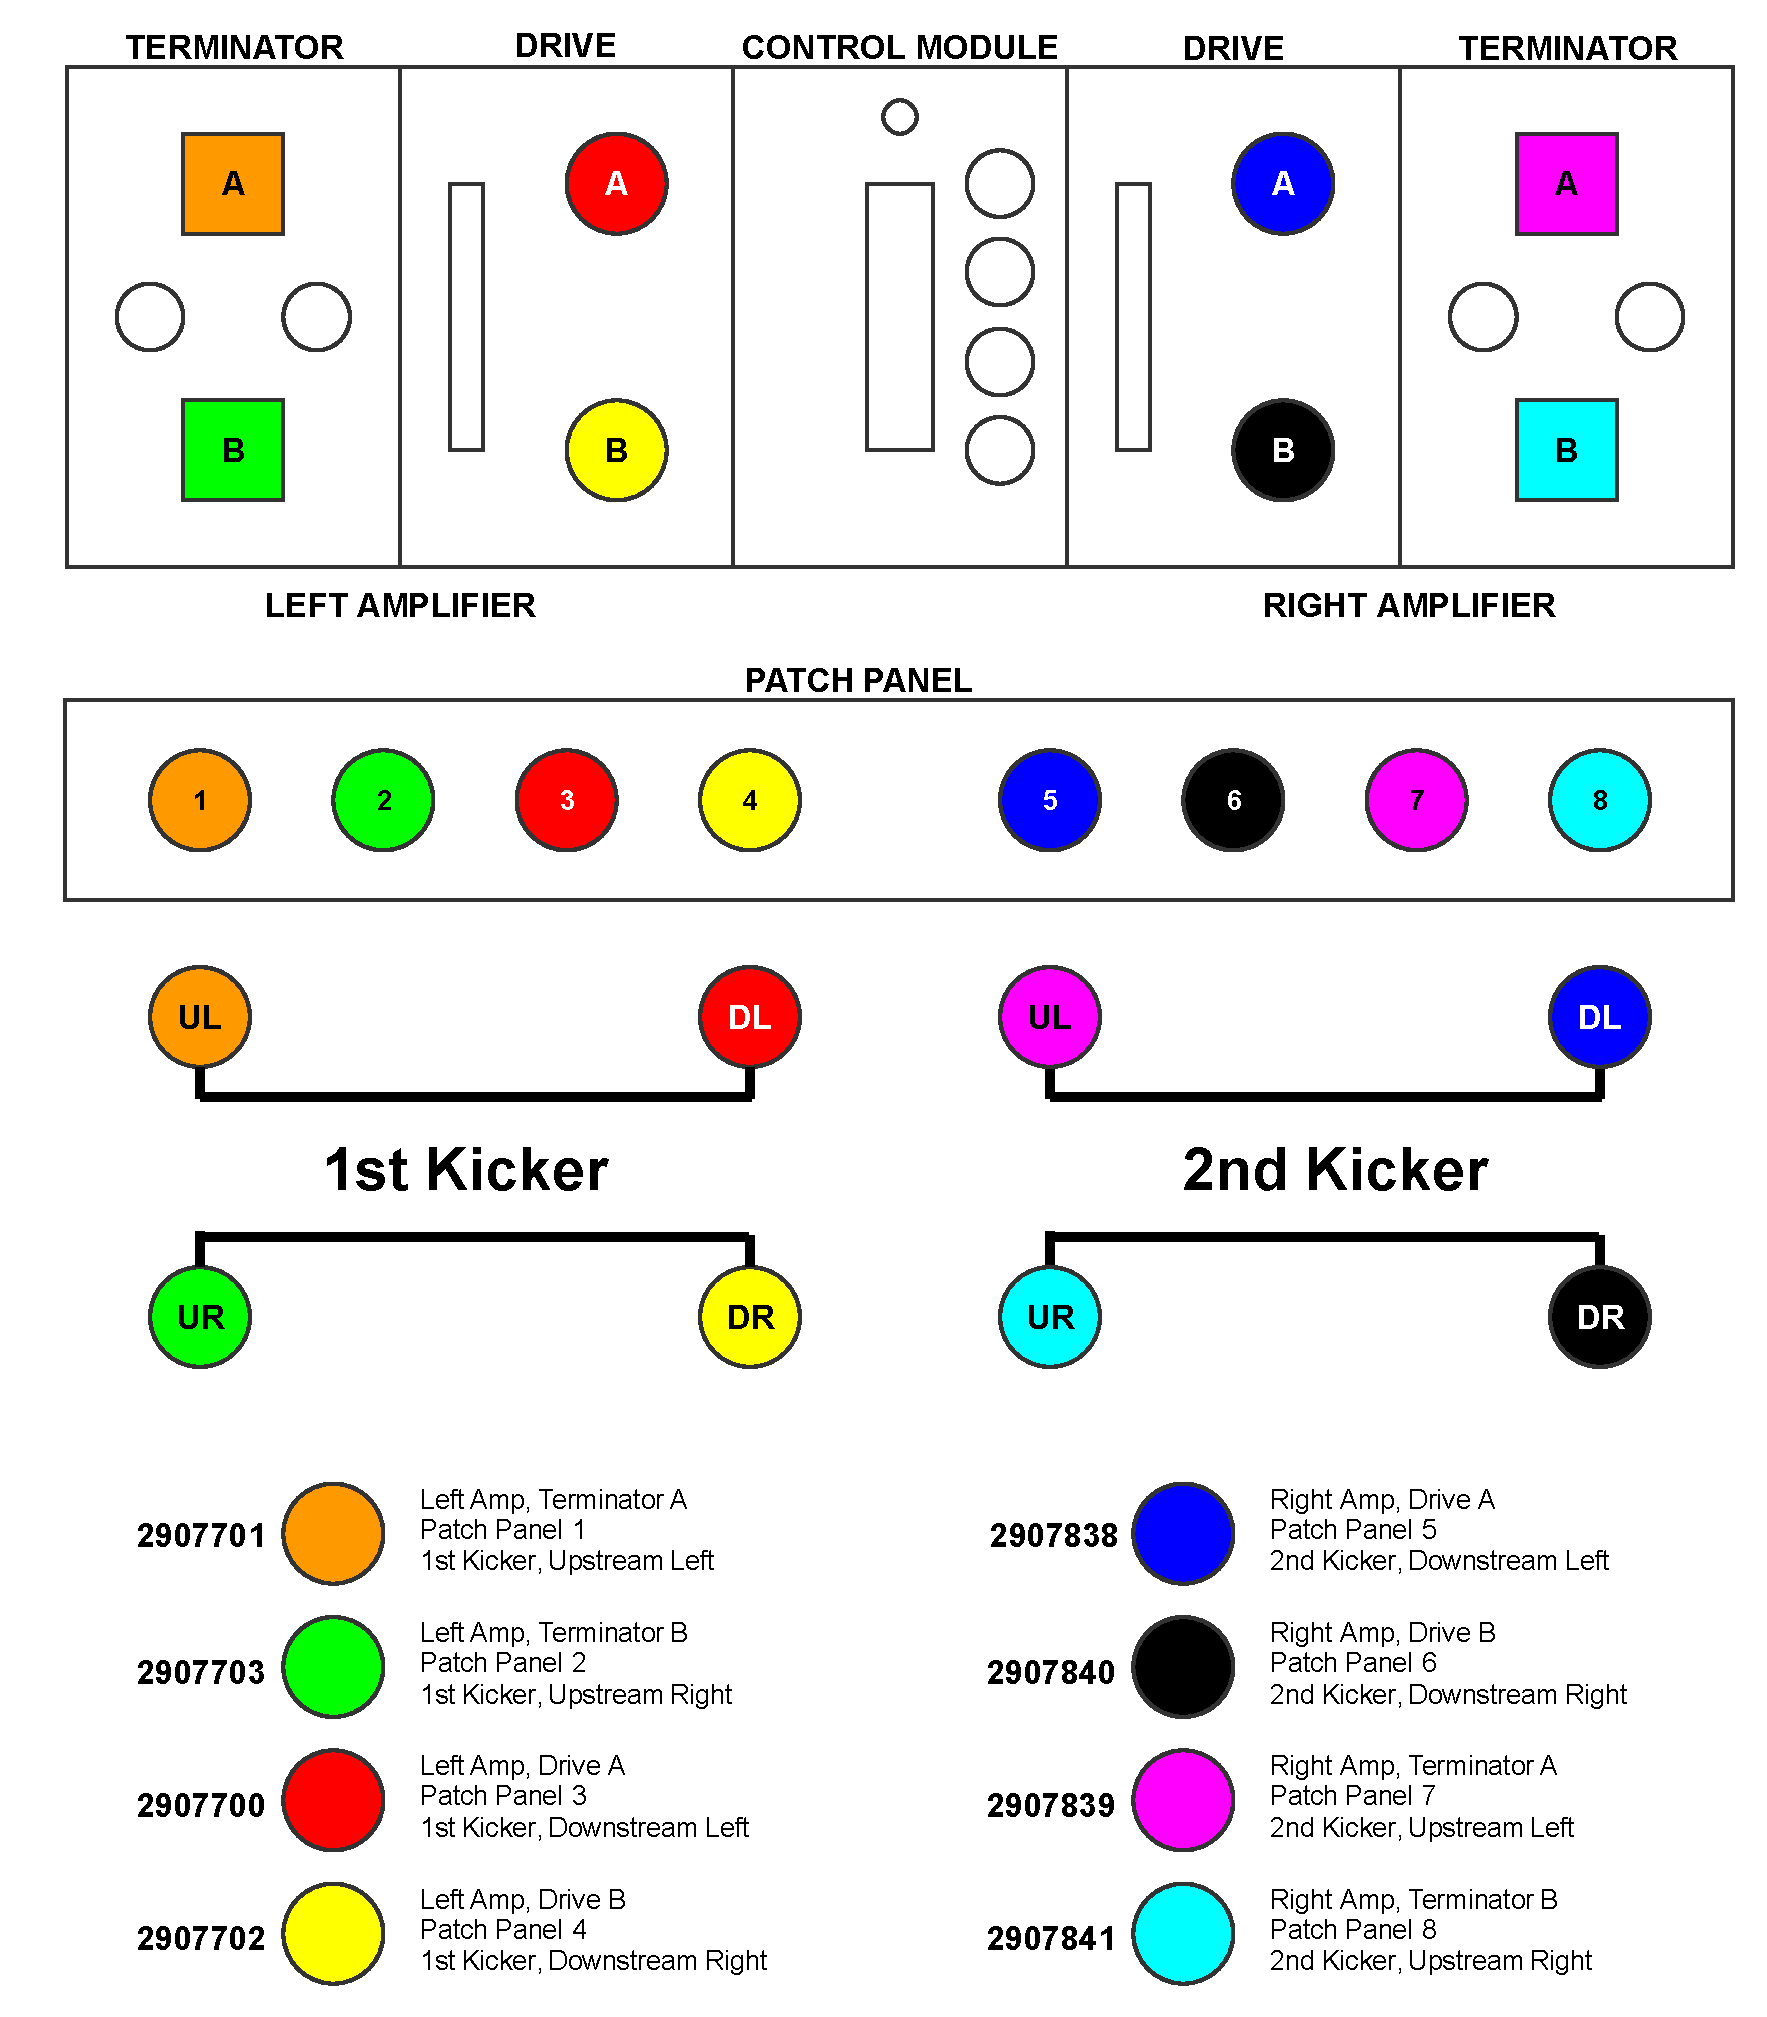
\includegraphics[width=\textwidth]{Figures/commissioning/kickerCables}
  \caption{Cable connections between the amplifier, patch panel and kickers.}
  \label{f:kickerCables}
\end{figure}

The patch panel cables all have lengths of around 3~ns, with the lengths of each matched to within the measurement error. After the re-routing and shortening of the kicker cables the cables connected to the first kicker have a length of around \(170\)~ns, whilst the cables for the downstream kicker are longer at around \(205\)~ns. For the downstream kicker the latency requirements are slightly relaxed due to the additional 36~ns beam time of flight between the kickers. Rather than also shortening the downstream kicker cables as much as possible some additional slack was left so that the difference in lengths is similar to the difference in the beam time of flight between the two. This means the two correction outputs (one for each kicker) can be sent from the FONT5a board at, or close to, the same time as discussed in Section~\ref{ss:relativeTiming}.

The pairs of cables connected to the downstream ends of the strips for
 each kicker have lengths matched within the measurement error.
 However, for the pairs connected to the upstream ends there are some differences, with cable 2907741A more than 1~ns shorter than cable 2907740A, for example. If there is a difference between the lengths of the cables connected to the downstream left and downstream right strips of a kicker (the driven end) there will be a time offset in the voltage applied to each side of the kicker, which would degrade the quality of the PFF correction. However, there is no need for the cables connected to the upstream ends of the kickers to be of matched lengths, the only requirement is that they are terminated correctly at the amplifier. The shorter 2907741A cable is therefore connected to the upstream end of the second kicker, and the cables 2907838A and 2907740A, with lengths matched to within 200~ps, are used to carry the amplifier output to the downstream end of the strips.


\subsection{Absolute Timing}
\label{ss:absTiming}



\subsubsection{Using Beam Pickup}
\label{sss:beamPickup}

Figure~\ref{f:beamPickup_noKick} shows the beam pickup at the start and end of the pulse from the PFF kickers at CTF3, as seen on one of the amplifier monitoring outputs (each of the four amplifier monitoring outputs, one for the upstream end of each strip prior to the signal being terminated at the amplifier, gives a similar response). The separation of the peaks in the beam pickup is \(1.1~\mathrm{\mu s}\), thus the same as the CTF3 pulse length as expected. By comparing the timing of these peaks with respect to the start and end of the amplifier output pulse, using the same amplifier monitoring signal, it is possible to ensure that the correction output arrives in sync with the beam.

\begin{figure}
  \centering
  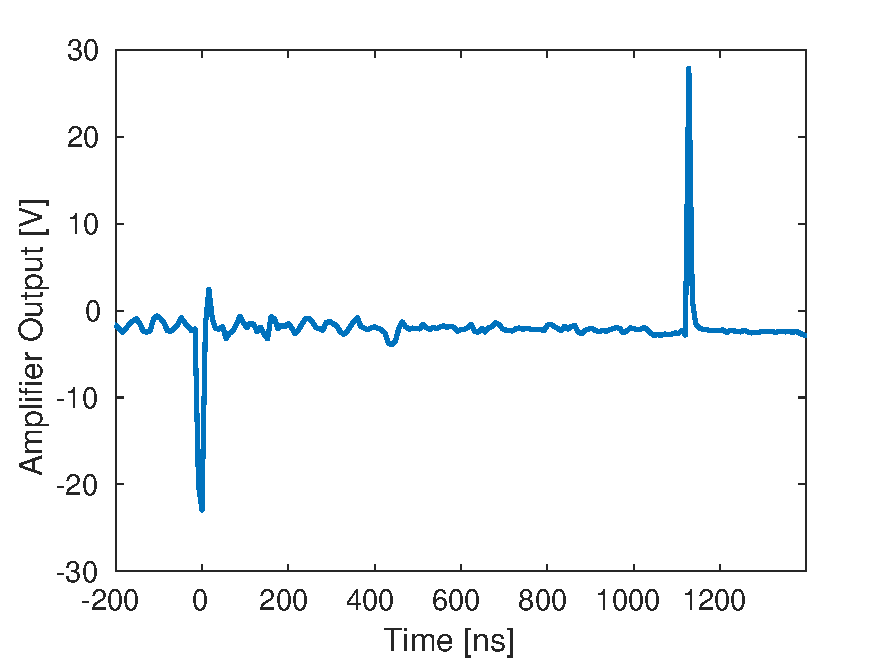
\includegraphics[width=0.75\textwidth]{Figures/commissioning/beamPickup_noKick}
  \caption{Beam pickup on the kicker strips as seen on amplifier monitoring signals.}
  \label{f:beamPickup_noKick}
\end{figure}

An example of this is shown in Figure~\ref{f:absDelay0_all}. A constant DAC output is used to drive the amplifier and both the resulting amplifier output pulse and the beam pickup, at samples 275 and 493, are visible in the figure. Importantly, the DAC output is gated using the upstream phase monitor diode signal (in other words, the constant DAC output is only enabled during the time when the diode is non-zero) and this has two consequences. Firstly, the amplifier output pulse has the same length as the beam pulse in the upstream phase monitor. Secondly, the timing of the output is identical to what it would be in normal PFF operation. In the case of Figure~\ref{f:absDelay0_all} the drive to the amplifier is applied as quickly as possible after the arrival of the upstream diode signal at the FONT5a board. It can be seen that the amplifier pulse arrives before the beam pickup, thus with the PFF system setup this way the correction would be applied slightly early. This result therefore proves that the PFF system just meets the latency requirements, with the overall time needed to transport and process all the relevant signals a few tens of nanoseconds less than the 380~ns time of flight of the beam between the upstream phase monitor and the first kicker. However, what is also clear in the figure is that the time offset between the start of the amplifier pulse and the first beam pickup spike is much larger than the time difference between the end of the amplifier pulse and the second beam pickup spike. This is due to the energy transient across the first 100~ns of the CTF3 beam pulse which is present in the upstream phase monitor but is then lost prior to the TL2 chicane, predominantly in TL1. As a result the downstream beam pulse is shorter than the upstream beam pulse which defines the length of the correction output. Therefore, in order to align the correction output with the beam the signals from the end of the amplifier and beam pulses must be used, not the start.

\begin{figure}
  \centering
  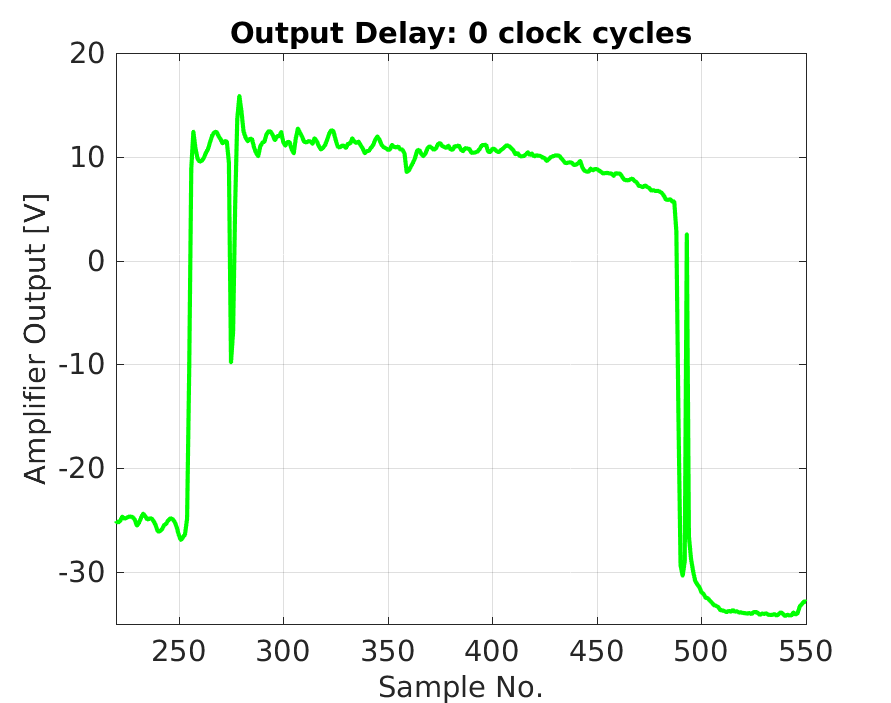
\includegraphics[width=0.8\textwidth]{Figures/commissioning/absDelay0_all}
  \caption{Alignment between the amplifier output (square pulse) and the beam pickup on the kickers strips (spikes) for an applied output delay of 0~ns (0 clock cycles).}
  \label{f:absDelay0_all}
  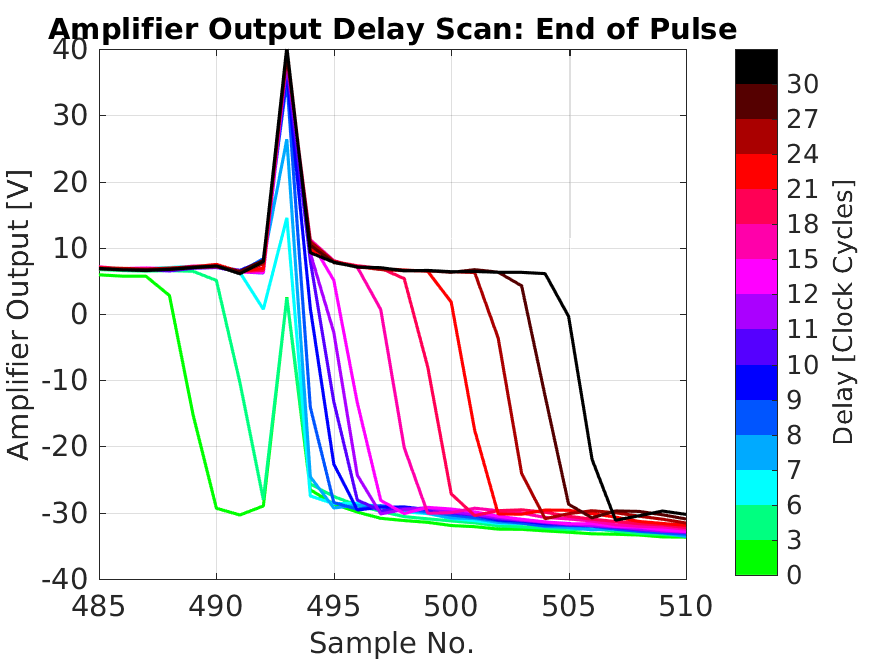
\includegraphics[width=0.75\textwidth]{Figures/commissioning/absDelayAll_endPulse}
  \caption{Alignment between the amplifier output (square pulse) and the beam pickup on the kickers strips (spikes) across the full range of possible output delays (as indicated by the colour scale).}
  \label{f:absDelayAll_endPulse}
\end{figure}

The firmware for the FONT5a board includes an output delay parameter that can be used to fine-tune the timing of the correction output sent to the amplifier (Section~\ref{ss:pffFirmware}). This can be done independently for each of the two correction outputs so that it can be ensured the correction arrives in sync with the beam in each kicker individually (the relative timing of the two kickers is discussed in the Section~\ref{ss:relativeTiming}). The delay can be varied between 0~and~31~clock~cycles in integer steps, with one clock cycle corresponding to one period of the 357~MHz ADC clock frequency, or 2.8~ns. A delay of up to 86.8~ns can therefore be added to the correction outputs. Figure~\ref{f:absDelayAll_endPulse} shows the effect of varying the output delay across the full range of possible values, zoomed in on the end of the pulse. For all output delays the beam pickup remains at sample 493, as expected. Meanwhile, the end of the amplifier pulse is moved from before the beam pickup (output too early) to after the beam pickup (output too late). To achieve the optimal correction timing the end of the amplifier pulse must be aligned with the beam pickup and this is achieved with a delay of 7~clock~cycles, or 19.6~ns, as shown in Figures~\ref{f:absDelay7_all}~and~\ref{f:absDelay7_end}. This delay has been used for the latest PFF runs presented in Chapter~\ref{c:feedforward}. Due to ambiguity in which point along the falling edge of the amplifier pulse the beam pickup should be aligned to there may be a remaining error of up 3 clock cycles in the exact alignment, and this can only be verified by beam based measurements (not using the amplifier monitoring outputs). 

\begin{figure}
  \centering
  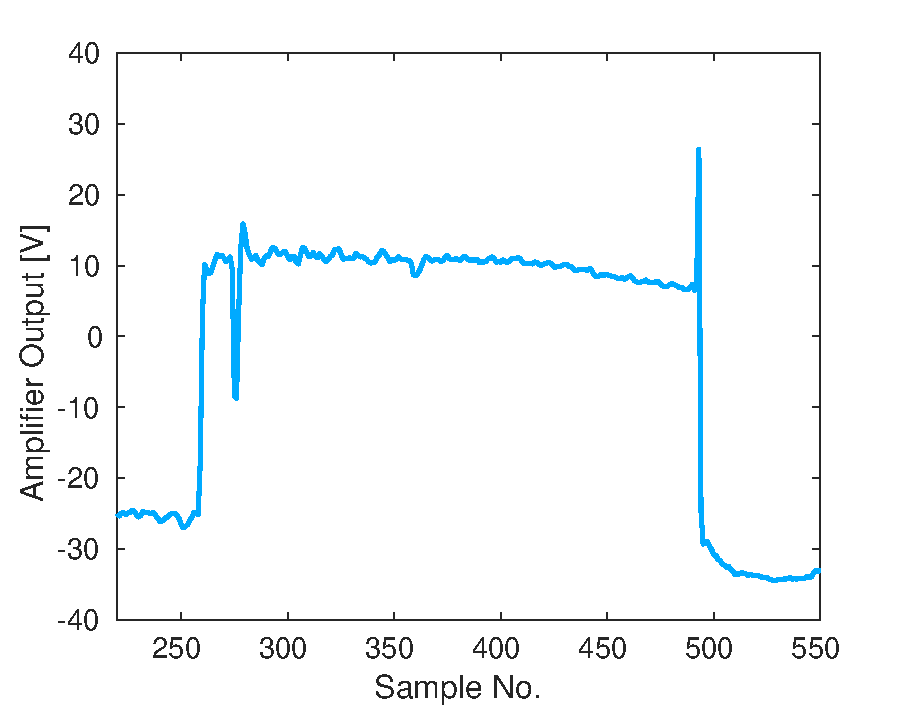
\includegraphics[width=0.75\textwidth]{Figures/commissioning/absDelay7_all}
  \caption{Alignment between the amplifier output (square pulse) and the beam pickup on the kickers strips (spikes) for an applied output delay of 19.6~ns (7 clock cycles).}
  \label{f:absDelay7_all}
  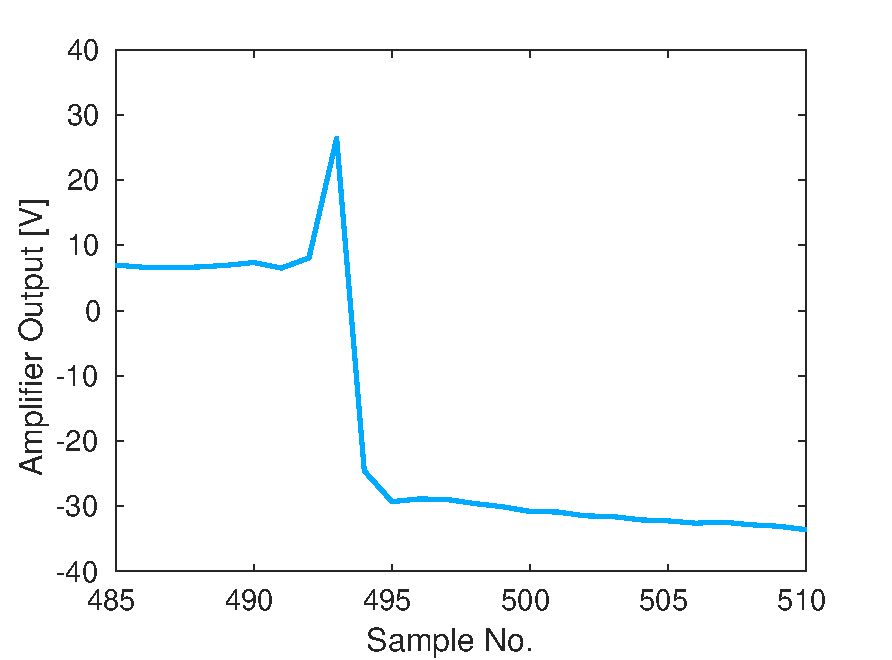
\includegraphics[width=0.75\textwidth]{Figures/commissioning/absDelay7_end}
  \caption{Alignment between the amplifier output (square pulse) and the beam pickup on the kickers strips (spikes) for an applied output delay of 19.6~ns (7 clock cycles), zoomed in to the end of the pulse.}
  \label{f:absDelay7_end}
\end{figure}


\subsubsection{Using BPMs}
\label{sss:relativeBPM}

This section presents one way in which the correction output timing can be determined using a combination of the phase monitor measurements and a BPM signal downstream of the TL2 chicane. The results shown here were performed with the first, lower power version of the amplifier and the FONT5 rather than the later FONT5a board, and because of this the optimal output delay calculated here does not agree with the value of 7~clock~cycles from the beam pickup based measurement above. The newer hardware has the same latency as the previous versions, thus the difference does not come from hardware changes but rather associated changes to cabling between the phase monitor electronics, FONT5a board and amplifier. The measurement will be repeated in the future to verify that both methods give consistent results when the same hardware and cabling setup is used.

The FONT5 (and FONT5a) board firmware provides the functionality to be able to change the gain of each PFF correction output independently. This means it is possible to apply the correction to only one kicker, or to kick the beam in the same direction in each kicker (i.e. to use the same sign for the gain in each kicker, rather than gains with equal magnitude but opposite sign). In both of these cases the kicked PFF orbit in the chicane is not closed, thus the horizontal position along the beam pulse in a BPM after the chicane depends on the shape and timing of the applied correction.\footnote{In Section~\ref{ss:orbitClosure} it was shown that the corrected orbit is not perfectly closed in normal PFF operation either. However, in this case no attempt at orbit closure is made so the measured effect seen in the BPMs is much larger.}

Figure~\ref{f:absTimBeam_d0} compares the upstream phase, downstream phase and horizontal position (in a BPM after the TL2 chicane) along the pulse in the case where the PFF correction is applied with gains set to kick the beam in the same direction in each kicker, and with no output delay applied in the FONT5 board. The data is taken in interleaved mode, with the plotted phases shown using the PFF off data and the BPM trace being the difference between the PFF on and PFF off data. Each signal is scaled and sign flipped where necessary to give variations along the pulse with the same magnitude and sign, in arbitrary units. The BPM and phase monitor signals are acquired with the same sampling frequency of 192~MHz, with each aligned so that the end of the pulse is at the same sample number. 

By taking the difference of the PFF off and PFF on data in the BPM any residual orbit variations along the pulse not related to the PFF system are removed, thus the remaining shape should match that of the PFF correction output, which in turn is linked to the upstream phase. The downstream phase should also have the same shape as the upstream phase with the PFF system off, within the limits of the upstream-downstream phase correlation achieved at this time. During this measurement many oscillations along the upstream phase were present, which usually are not desired but for this measurement are perfect points of reference to check the time alignment of the signals. As expected the overall shape of the residual horizontal position in the BPM along the pulse and the two phase signals is very similar. The largest feature in the upstream phase that is present in all three signals occurs at sample 671 in the upstream phase, with the location of the peak of this oscillation in the phase signals and the BPM marked by vertical black lines in the figure. The peak as seen in the BPM signal is clearly before the peak in the phase monitor signals thus in this case the correction was applied early, with a measured offest of -36~ns between the peaks.

\begin{figure}
  \centering
  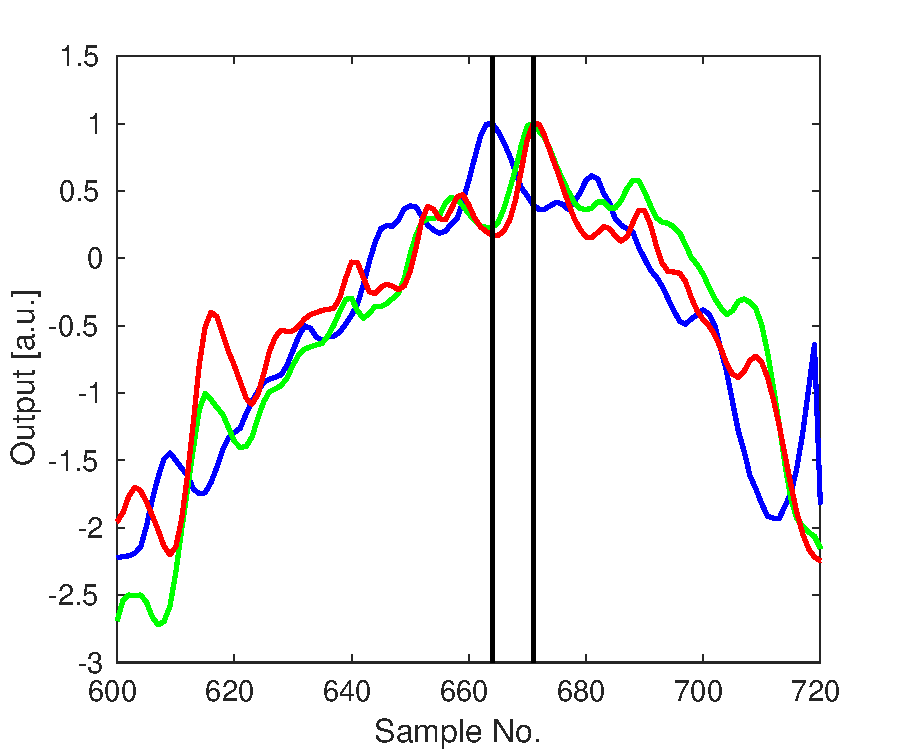
\includegraphics[width=0.75\textwidth]{Figures/commissioning/absTimBeam_d0}
  \caption{Alignment of the upstream (green) and downstream (red) phase compared to the applied kick as measured in a BPM after the TL2 chicane (blue) for an output delay of 0~ns. Vertical black lines indicate the time shift between the phase and the kick for the clearest feature visible in all three signals.}
  \label{f:absTimBeam_d0}
  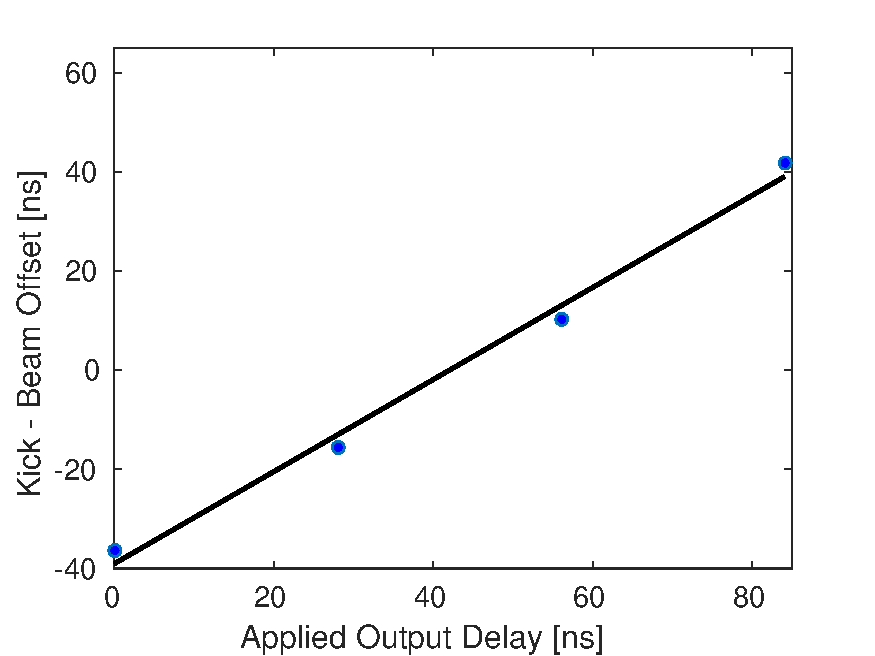
\includegraphics[width=0.75\textwidth]{Figures/commissioning/absTimBeam_fit}
  \caption{Fitted time offset between the applied kick and the beam at different output delays.}
  \label{f:absTimBeam_fit}
\end{figure}

\begin{figure}
  \centering
  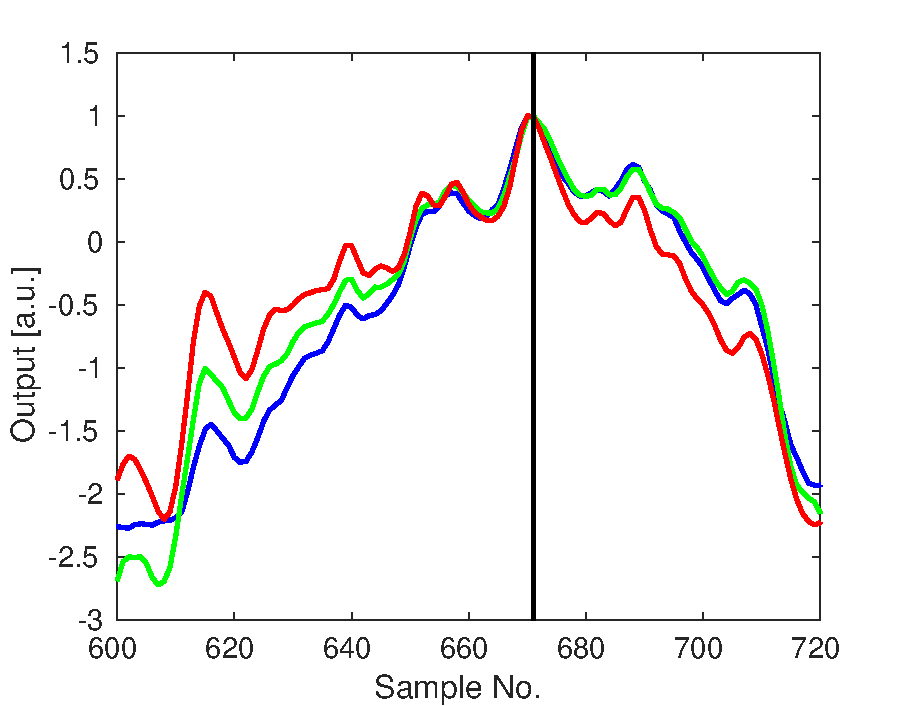
\includegraphics[width=0.75\textwidth]{Figures/commissioning/absTimBeam_opt}
  \caption{Alignment between the applied kick as measured by a BPM after the chicane (blue) and the phase signals (red downstream and green upstream) after applying the optimal output delay in data analysis.}
  \label{f:absTimBeam_opt}
\end{figure}

This measurement was repeated with four different correction output delays applied in the FONT5 board, at delays of 0, 10, 20 and 30~clock~cycles (0 to 84~ns), which includes points where the correction is applied both early and late. Fitting the measured time offset between the peaks in the BPM and the phase in the same way as before yields an optimal correction output delay to apply of \(39\pm7\)~ns (Figure \ref{f:absTimBeam_fit}), or \(14\pm3\)~clock~cycles. Applying this delay in data analysis offline gives the result shown in Figure~\ref{f:absTimBeam_opt}, in which the similarity of the three signals becomes clear.

\subsection{Relative Kicker Timing}
\label{ss:relativeTiming}

For the phase correction the absolute output timing sent to the first kicker, as derived above, is the most critical as this defines the alignment of the applied phase shift in the chicane with the beam. The second kicker's main purpose is then to close the kick created by the first, ensuring the orbit after the chicane is closed (with the caveats already mentioned in Section~\ref{ss:orbitClosure}). For the purposes of orbit closure it is also important to ensure that the correction arrives at the second kicker in time with the beam. As discussed in Section~\ref{ss:kickerCables} the beam time of flight between the kickers is about 36~ns, thus the correction must arrive at the second kicker 36~ns later than the first kicker. Most of this difference should be accounted for by the longer cable lengths for the second kicker, but the precise relative timing is checked here. In this context the relative timing means the additional output delay that must be applied to the FONT5a correction output for the second kicker with respect to the first in order to ensure the correction is aligned in time with the beam in both kickers.

Figure~\ref{f:relDelay_sim} shows a simulated example of the expected effect of kicking the beam with a relative time offset in each kicker, in this case with the output to the second kicker arriving later than the first kicker (with respect to the beam pulse). The kickers are driven with opposite polarity in the same way as the PFF system, and the first kicker is shown with a larger output than the second. The total kick received in the chicane is given by the sum of the two, as shown in the figure. In the ideal case the total/residual kick in the chicane should be zero so that the orbit is closed after the chicane. However, with a timing offset between the two kickers there are large peaks in the residual kick at the start and end of the pulse, where only one of the two kickers receives its full drive. Due to the different amplitude of the two kickers the residual kick is also non-zero in the central part of the pulse. With well-aligned timing the residual kick would be constant along the full pulse length, or zero across the full pulse length if the kicks had matched amplitudes.

\begin{figure}
  \centering
  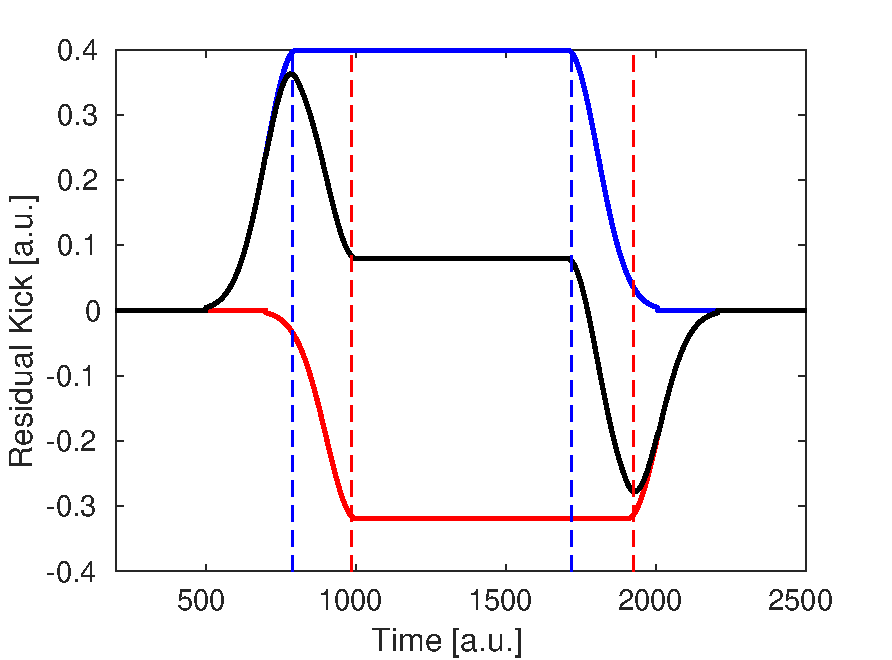
\includegraphics[width=0.75\textwidth]{Figures/commissioning/relDelay_sim}
  \caption{Example of the residual kick (black) experienced by a beam traversing through two kickers. A relative delay between the applied output to each kicker is applied, as well as a different magnitude kick from each kicker (shown in blue and red). Dashed blue and red lines show the kick start and end time for each kicker.}
  \label{f:relDelay_sim}
\end{figure}

By varying the relative timing of the two correction outputs on the FONT5a board (K1 and K2 delay, see Section~\ref{ss:pffFirmware}) and using a BPM after the TL2 chicane to measure the size of the peaks at the start and end of the pulse resulting from the offset kicks (in the same way as Figure~\ref{f:relDelay_sim}) the optimal relative delay can be determined. The optimal relative delay is the point that minimises the size of the peaks on the rising/falling edge of the pulse, with the peak magnitude  approximately linearly dependent on the delay. Figure~\ref{f:relDelay_traces} shows the result of doing this, using a constant DAC output from the FONT5a board applied across a 168~ns portion of the pulse. The horizontal position in a BPM after the TL2 chicane is plotted for relative K2 delays ranging between -10 (K1 output delayed with respect to K2) to +10 (K2 output delayed with respect to K1) clock~cycles (-28~ns to +28~ns). Aside from the asymmetry between the size of the peaks at the start and end of the pulse the result is as expected from the example previously discussed. Note the non-zero position offset in the central part of the pulse. Based on the orbit closure results in Section~\ref{ss:orbitClosure} this is predominantly due to optics differences leading to a non-closed orbit, rather than the small difference in amplifier output voltage to each kicker.

\begin{figure}
  \centering
  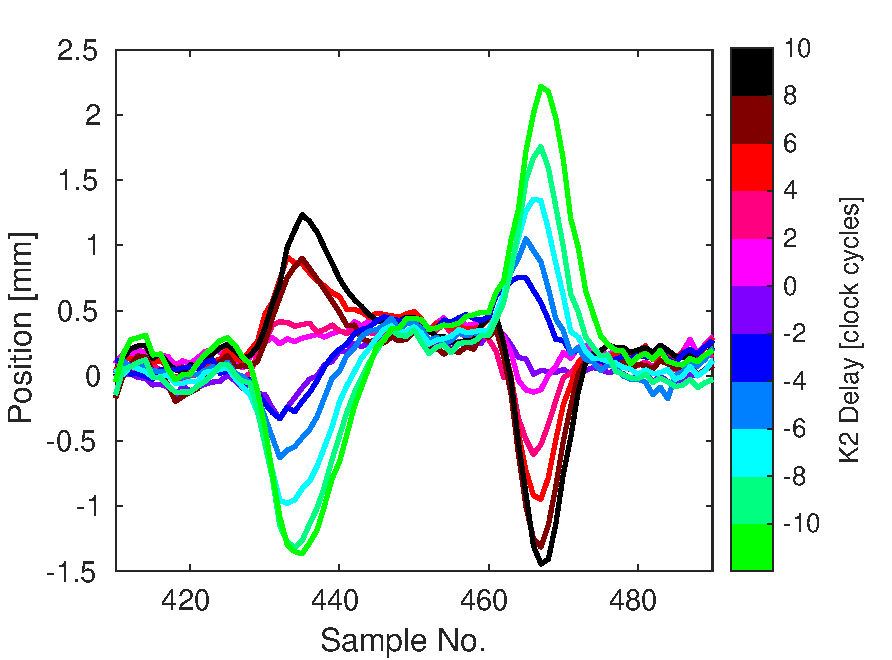
\includegraphics[width=0.75\textwidth]{Figures/commissioning/relDelay_traces}
  \caption{Measured position offset in a BPM after the chicane for different relative kick delays (as indicated by the colour scale).}
  \label{f:relDelay_traces}
\end{figure}

Figure~\ref{f:relDelay_fit} then shows the peak beam offset in the BPM versus the relative K2 delay. The peak beam offset is defined as the difference between the maximum and minimum beam position after the chicane between sample 425 and 447 for the rising edge, or sample 458 and 477 for the falling edge of the pulse (as seen in Figure~\ref{f:relDelay_traces}). As the K2 delay approaches the optimal value the difference in beam position in this range converges to the 0.3~mm offset in the flat central part of the kicked pulse. The point of intersection between the two linear fits shown (one for the points with a positive peak position and the other for points with a negative peak) gives the optimal relative K2 offset to be \(0.1\pm0.5\)~clock~cycles (\(0.3\pm1.4\)~ns) for the falling edge of the pulse. Repeating the procedure for the peaks at the rising edge of the pulse gives a result of \(1.9\pm2.0\)~clock~cycles (\(5.3\pm5.6\)~ns), and the two results combine to give an optimal value of \(0.5\pm0.6\)~clock~cycles (\(1.4\pm1.7\)~ns).

\begin{figure}
  \centering
  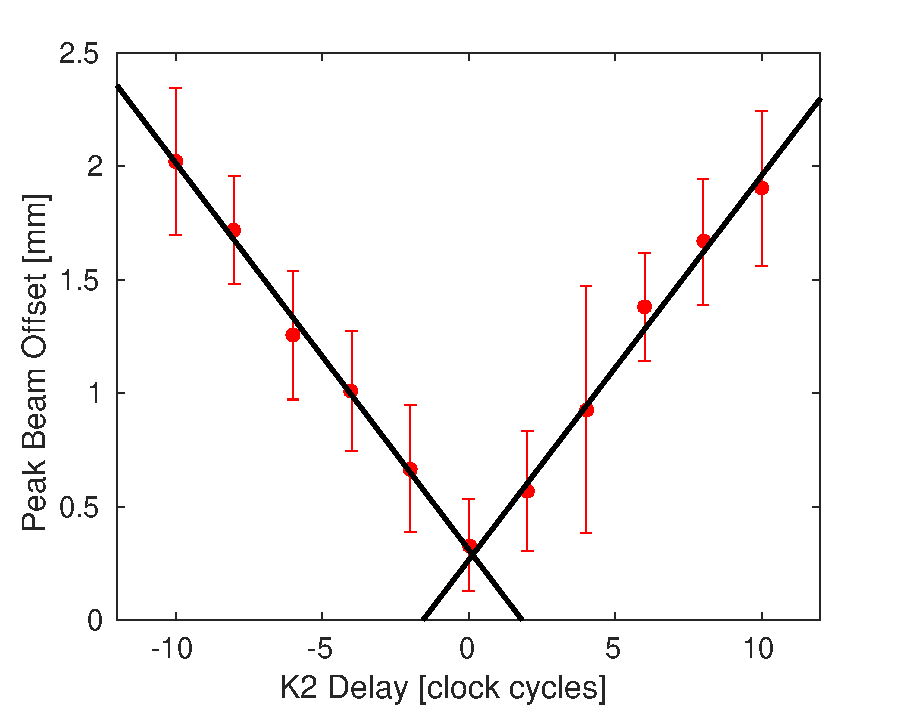
\includegraphics[width=0.75\textwidth]{Figures/commissioning/relDelay_fit}
  \caption{Fitted peak position offset after the chicane vs. the applied relative kick delay. Fits to the peaks at both the rising edge (blue) and falling edge (red) of the pulse are shown. Dashed vertical lines show the fitted optimal delay in each case.}
  \label{f:relDelay_fit}
\end{figure}

Relative K2 delays of both 0 and 1 clock~cycles have been used during PFF operation, with no measurable difference in the PFF results between the two to date although this will have to be verified with further orbit closure tests. Adding the absolute delay of 7~clock~cycles derived in Section~\ref{ss:absTiming}, the final delays to apply in the FONT5a board are:
\begin{itemize}
\item \textbf{K1 delay}: 7 clock~cycles.
\item \textbf{K2 delay}: 7 or 8 clock~cycles.
\end{itemize}

%\newsection{earlyFFSim}{Early Phase Feedforward Attempts and Simulations}
%
%This is the introductory text.
%
%\subsection{Gain Scans}
%\label{ss:gainScans}
%
%\subsection{Effect of Limited Correction Range}
%\label{ss:effectLimRange}
%
